%%%%%%%%%%%%%%%%%%%%%%%%%%%%%%%%%%%%%%%%%%%%%%%%%%%%%%%%%%%%%%%%%%%%%%%%%%%%%%%%
%  Zawartość: Główny plik szablonu pracy dyplomowej (magisterskiej/inżynierskiej). 
%  Opracował: Tomasz Kubik <tomasz.kubik@pwr.edu.pl>
%  Data: styczeń 2023
%  Wersja: 0.9
%  Wymagania: kompilator pdflatex
%%%%%%%%%%%%%%%%%%%%%%%%%%%%%%%%%%%%%%%%%%%%%%%%%%%%%%%%%%%%%%%%%%%%%%%%%%%%%%%%

\documentclass[a4paper,onecolumn,oneside,12pt,extrafontsizes]{memoir}
%  W celu przygotowania wydruku do archiwum można:
%  a) przygotować pdf, w którym dwie strony zostaną wstawione na jedną fizyczną stronę i taki dokument wydrukować dwustronnie (podejście zalecane)
%
%   Taki dokument można przygotować poprzez
%   - wydruk z Adobe Acrobat Reader z opcją "Wiele" - sekcja "Rozmiar i obsługa stron"
%   - wykorzystanie narzędzi psutils
%
%      Windows (zakładając, że w dystrybucji MiKTeX jest pakiet miktex-psutils-bin-x64-2.9):
%        "c:\Program Files\MiKTeX 2.9\miktex\bin\x64\pdf2ps.exe" Dyplom.pdf Dyplom.ps
%        "c:\Program Files\MiKTeX 2.9\miktex\bin\x64\psnup.exe" -2 Dyplom.ps Dyplom2.ps
%        "c:\Program Files\MiKTeX 2.9\miktex\bin\x64\ps2pdf.exe" Dyplom2.ps Dyplom2.pdf
%        Del Dyplom2.ps Dyplom.ps
%
%     Linux:
%        pdf2ps Dyplom.pdf - | psnup -2 | ps2pdf - Dyplom2.pdf
%
%  b) przekomplilować dokument zmniejszając czcionkę (podejście niezalecane, bo zmienia formatowanie dokumentu)
%
%    Do tego wystarczy posłużyć się poniższymi komendami (zamiast documentclass z pierwszej linijki):
%   \documentclass[a4paper,onecolumn,twoside,10pt]{memoir} 
%   \renewcommand{\normalsize}{\fontsize{8pt}{10pt}\selectfont}

%\usepackage[cp1250]{inputenc} % Proszę zostawić, jeśli kodowanie edytowanych plików to cp1250 
\usepackage[utf8]{inputenc} % Proszę użyć zamiast powyższego, jeśli kodowanie edytowanych plików to UTF8
\usepackage[T1]{fontenc}
\usepackage[english,polish]{babel} % Tutaj ważna jest kolejność atrybutów (dla pracy po polsku polish powinno być na końcu)
%\DisemulatePackage{setspace}
\usepackage{setspace}
\usepackage{color,calc}
%\usepackage{soul} % pakiet z komendami do podkreślania, przekreślania, podświetlania tekstu (raczej niepotrzebny)
\usepackage{ebgaramond} % pakiet z czcionkami garamond, potrzebny tylko do strony tytułowej, musi wystąpić przed pakietem tgtermes

%% Aby uzyskać polskie literki w pdfie (a nie zlepki) korzystamy z pakietu czcionek tgterms. 
%% W pakiecie tym są zdefiniowane klony czcionek Times o kształtach: normalny, pogrubiony, italic, italic pogrubiony.
%% W pakiecie tym brakuje czcionki o kształcie: slanted (podobny do italic). 
%% Jeśli w dokumencie gdzieś zostanie zastosowana czcionka slanted (np. po użyciu komendy \textsl{}), to
%% latex dokona podstawienia na czcionkę standardową i zgłosi to w ostrzeżeniu (warningu).
%% Ponadto tgtermes to czcionka do tekstu. Wszelkie matematyczne wzory będą sformatowane domyślną czcionką do wzorów.
%% Jeśli wzory mają być sformatowane z wykorzystaniem innych czcionek, trzeba to jawnie zadeklarować.

%% Po zainstalowaniu pakietu tgtermes może będzie trzeba zauktualizować informacje 
%% o dostępnych fontach oraz mapy. Można to zrobić z konsoli (jako administrator)
%% initexmf --admin --update-fndb
%% initexmf --admin --mkmaps

\usepackage{tgtermes}   
\renewcommand*\ttdefault{txtt}


%%%%%%%%%%%%%%%%%%%%%%%%%%%%%%%%%%%%%%%%%%%%%%%%%%%%%%%%%%%%%%%%%%%%%%%%%%%%%%%%
%% Ustawienia odpowiedzialne za sposób łamania dokumentu
%% i ułożenie elementów pływających
%%%%%%%%%%%%%%%%%%%%%%%%%%%%%%%%%%%%%%%%%%%%%%%%%%%%%%%%%%%%%%%%%%%%%%%%%%%%%%%%
%\hyphenpenalty=10000		% nie dziel wyrazów zbyt często
\clubpenalty=10000      % kara za sierotki
\widowpenalty=10000     % nie pozostawiaj wdów
%\brokenpenalty=10000		% nie dziel wyrazów między stronami - trzeba było wyłączyć, bo nie łamały się linie w lstlisting
%\exhyphenpenalty=999999		% nie dziel słów z myślnikiem - trzeba było wyłączyć, bo nie łamały się linie w lstlisting
\righthyphenmin=3			  % dziel minimum 3 litery

%\tolerance=4500
%\pretolerance=250
%\hfuzz=1.5pt
%\hbadness=1450

\renewcommand{\topfraction}{0.95}
\renewcommand{\bottomfraction}{0.95}
\renewcommand{\textfraction}{0.05}
\renewcommand{\floatpagefraction}{0.35}

%%%%%%%%%%%%%%%%%%%%%%%%%%%%%%%%%%%%%%%%%%%%%%%%%%%%%%%%%%%%%%%%%%%%%%%%%%%%%%%%
%%  Ustawienia rozmiarów: tekstu, nagłówka i stopki, marginesów
%%  dla dokumentów klasy memoir 
%%%%%%%%%%%%%%%%%%%%%%%%%%%%%%%%%%%%%%%%%%%%%%%%%%%%%%%%%%%%%%%%%%%%%%%%%%%%%%%%
\setlength{\headsep}{10pt} 
\setlength{\headheight}{13.6pt} % wartość baselineskip dla czcionki 11pt tj. \small wynosi 13.6pt
\setlength{\footskip}{\headsep+\headheight}
\setlength{\uppermargin}{\headheight+\headsep+1cm}
\setlength{\textheight}{\paperheight-\uppermargin-\footskip-1.5cm}
\setlength{\textwidth}{\paperwidth-5cm}
\setlength{\spinemargin}{2.5cm}
\setlength{\foremargin}{2.5cm}
\setlength{\marginparsep}{2mm}
\setlength{\marginparwidth}{2.3mm}
%\settrimmedsize{297mm}{210mm}{*}
%\settrims{0mm}{0mm}	
\checkandfixthelayout[fixed] % konieczne, aby się dobrze wszystko poustawiało
%%%%%%%%%%%%%%%%%%%%%%%%%%%%%%%%%%%%%%%%%%%%%%%%%%%%%%%%%%%%%%%%%%%%%%%%%%%%%%%%
%%  Ustawienia odległości linii, wcięć, odstępów
%%%%%%%%%%%%%%%%%%%%%%%%%%%%%%%%%%%%%%%%%%%%%%%%%%%%%%%%%%%%%%%%%%%%%%%%%%%%%%%%
\linespread{1}
%\linespread{1.241}
\setlength{\parindent}{14.5pt}


\usepackage{multicol} % pakiet umożliwiający stworzenie wielokolumnowego tekstu
%%%%%%%%%%%%%%%%%%%%%%%%%%%%%%%%%%%%%%%%%%%%%%%%%%%%%%%%%%%%%%%%%%%%%%%%%%%%%%%%
%% Pakiety do formatowania tabel
%%%%%%%%%%%%%%%%%%%%%%%%%%%%%%%%%%%%%%%%%%%%%%%%%%%%%%%%%%%%%%%%%%%%%%%%%%%%%%%%
\usepackage{tabularx}
% Proszę używać tylko tabularx. Innych pakietów proszę nie stosować !!!
% Dokument na pewno da się zredagować bez ich użycia.
%\usepackage{longtable}
%\usepackage{ltxtable}
%\usepackage{tabulary}

%%%%%%%%%%%%%%%%%%%%%%%%%%%%%%%%%%%%%%%%%%%%%%%%%%%%%%%%%%%%%%%%%%%%%%%%%%%%%%%%
%% Pakiet do wstawiania fragmentów kodu
%%%%%%%%%%%%%%%%%%%%%%%%%%%%%%%%%%%%%%%%%%%%%%%%%%%%%%%%%%%%%%%%%%%%%%%%%%%%%%%%
\usepackage{listings} 
\usepackage{xpatch}
\makeatletter
\xpatchcmd\l@lstlisting{1.5em}{0em}{}{}
\makeatother
% Pakiet dostarcza otoczenia lstlisting. Jest ono wysoce konfigurowalne. 
% Konfigurować można indywidualnie każdy z listingów lub globalnie, w poleceniu \lstset{}.

% Zalecane jest, by kod źródłowy był wyprowadzany z użyciem czcionki maszynowej \ttfamily
% Ponieważ kod źródłowy, nawet po obcięciu do interesujących fragmentów, bywa obszerny, należy zmniejszyć czcionkę.
% Zalecane jest \small (dla krótkich fragmentów) oraz \footnotesize (dla dłuższych fragmentów).

% Ponadto podczas konfiguracji można zadeklarować sposób numerowania linii. Numerowanie linii zalecane jest jednak 
% tylko w przypadkach, gdy w redagowanym tekście znajdują się jakieś odwołania do konkretnych linii.
% Jeśli takich odwołań nie ma, numerowanie linii jest zbędne. Proszę wtedy go nie stosować.
% Przy włączaniu numerowania linii należy zwrócić uwagę na to, gdzie pojawią się te numery.
% Bez zmiany dodatkowych parametrów pojawiają się one na marginesie strony (co jest niepożądane).

\lstset{
  basicstyle=\small\ttfamily, % lub basicstyle=\footnotesize\ttfamily
  language=C++,
  tabsize=4,
  %%columns=fullflexible,
	%%showstringspaces=false,
	%%showspaces=false,
  breaklines=true,
  breakatwhitespace=true,
  postbreak=\mbox{\textcolor{red}{$\hookrightarrow$}\space}, 
  %%numbers=left,  % ta i poniższe linie dotyczą ustawienia numerowania i sposobu jego wyprowadzania
  %%firstnumber=1, 
  %%numberfirstline=true, 
	%%xleftmargin=17pt,
  %%framexleftmargin=17pt,
  %%framexrightmargin=5pt,
  %%framexbottommargin=4pt,
	belowskip=.5\baselineskip,
	literate={\_}{{\_\allowbreak}}1 % ta deklaracja przydaje się, jeśli na listingu mają być łamane nazwy zawierające podkreślniki
}

% Jeśli edytowany plik nie jest w kodowaniu cp1250, to jest problem z polskimi znakami występującymi we wstawianym kodzie.
% Dlatego podczas pracy na plikach w kodowaniu UTF8 trzeba zadeklarować mapowanie jak niżej (wystarczy odmarkować).
% Niestety, jak się zastosuje to mapowanie mogą pojawić się problemy z podświetlaniem składni (patrz dalej).
\lstset{literate=%-
{ą}{{\k{a}}}1 {ć}{{\'c}}1 {ę}{{\k{e}}}1 {ł}{{\l{}}}1 {ń}{{\'n}}1 {ó}{{\'o}}1 {ś}{{\'s}}1 {ż}{{\.z}}1 {ź}{{\'z}}1 {Ą}{{\k{A}}}1 {Ć}{{\'C}}1 {Ę}{{\k{E}}}1 {Ł}{{\L{}}}1 {Ń}{{\'N}}1 {Ó}{{\'O}}1 {Ś}{{\'S}}1 {Ż}{{\.Z}}1 {Ź}{{\'Z}}1 
    {Ö}{{\"O}}1
    {Ä}{{\"A}}1
    {Ü}{{\"U}}1
    {ß}{{\ss}}1
    {ü}{{\"u}}1
    {ä}{{\"a}}1
    {ö}{{\"o}}1
    {~}{{\textasciitilde}}1
		{—}{{{\textemdash} }}1
}%{\ \ }{{\ }}1}


%% lstlisting pozwala na ostylowania podświetlania składni wybranych języków.
%% Działa to na zasadzie zdefiniowania słów kluczowych oraz sposobu ich wyświetlania.
%% Ponieważ jest to prosty mechanizm, czasem trudno osiągnąć takie efekty, jakie dają narzędzia IDE. 
%% Jednak w większości przypadku osiągane rezutlaty są zadowalające.


%% lstlisting obsługuje domyślnie kilka najpopularniejszych języków.
%%\lstloadlanguages{% Check Dokumentation for further languages ...
%%C,
%%C++,
%%csh,
%%Java
%%}
%% Inne języki muszą być dodefiniowane. Poniżej podano przykłady definicji języków i styli.

\definecolor{lightgray}{rgb}{.9,.9,.9}
\definecolor{darkgray}{rgb}{.4,.4,.4}
\definecolor{purple}{rgb}{0.65, 0.12, 0.82}
\definecolor{javared}{rgb}{0.6,0,0} % for strings
\definecolor{javagreen}{rgb}{0.25,0.5,0.35} % comments
\definecolor{javapurple}{rgb}{0.5,0,0.35} % keywords
\definecolor{javadocblue}{rgb}{0.25,0.35,0.75} % javadoc
 
\lstdefinelanguage{JavaScript}{ 
	keywords={typeof, new, true, false, catch, function, return, null, catch, switch, var, if, in, while, do, else, case, break},
	keywordstyle=\color{blue}\bfseries,
	ndkeywords={class, export, boolean, throw, implements, import, this},
	ndkeywordstyle=\color{darkgray}\bfseries,
	identifierstyle=\color{black},
	sensitive=false,
	comment=[l]{//},
	morecomment=[s]{/*}{*/},
	commentstyle=\color{purple}\ttfamily,
	stringstyle=\color{red}\ttfamily,
	morestring=[b]',
	morestring=[b]"
}
\lstdefinestyle{JavaScriptStyle}{
	language=JavaScript,
	commentstyle=\color{javagreen}, % niestety, jeśli w linii komentarza pojawią się słowa kluczowe, to zostaną pokolorowane
	backgroundcolor=,%\color{lightgray}, % można ustwić kolor tła, ale jest to niezalecane
	extendedchars=true,
	basicstyle=\footnotesize\ttfamily,
	showstringspaces=false,
	showspaces=false,
	numbers=none,%left,
	numberstyle=\footnotesize,
	numbersep=9pt,
	tabsize=2,
	breaklines=true,
	showtabs=false,
	captionpos=t
}

\lstdefinestyle{JavaStyle}{
basicstyle=\footnotesize\ttfamily,
keywordstyle=\color{javapurple}\bfseries,
stringstyle=\color{javared},
commentstyle=\color{javagreen},
morecomment=[s][\color{javadocblue}]{/**}{*/},
numbers=none,%left,
numberstyle=\tiny\color{black},
stepnumber=2,
numbersep=10pt,
tabsize=4,
showspaces=false,
showstringspaces=false,
captionpos=t
}

\definecolor{pblue}{rgb}{0.13,0.13,1}
\definecolor{pgreen}{rgb}{0,0.5,0}
\definecolor{pred}{rgb}{0.9,0,0}
\definecolor{pgrey}{rgb}{0.46,0.45,0.48}
\definecolor{dark-grey}{rgb}{0.4,0.4,0.4}
% styl json
\newcommand\JSONnumbervaluestyle{\color{blue}}
\newcommand\JSONstringvaluestyle{\color{red}}

\newif\ifcolonfoundonthisline

\makeatletter

\lstdefinestyle{json-style}  
{
	showstringspaces    = false,
	keywords            = {false,true},
	alsoletter          = 0123456789.,
	morestring          = [s]{"}{"},
	stringstyle         = \ifcolonfoundonthisline\JSONstringvaluestyle\fi,
	MoreSelectCharTable =%
	\lst@DefSaveDef{`:}\colon@json{\processColon@json},
	basicstyle          = \footnotesize\ttfamily,
	keywordstyle        = \ttfamily\bfseries,
	numbers				= left, % zakomentować, jeśli numeracja linii jest niepotrzebna
	numberstyle={\footnotesize\ttfamily\color{dark-grey}},
	xleftmargin			= 2em % zakomentować, jeśli numeracja linii jest niepotrzebna
}

\newcommand\processColon@json{%
	\colon@json%
	\ifnum\lst@mode=\lst@Pmode%
	\global\colonfoundonthislinetrue%
	\fi
}

\lst@AddToHook{Output}{%
	\ifcolonfoundonthisline%
	\ifnum\lst@mode=\lst@Pmode%
	\def\lst@thestyle{\JSONnumbervaluestyle}%
	\fi
	\fi
	\lsthk@DetectKeywords% 
}

\lst@AddToHook{EOL}%
{\global\colonfoundonthislinefalse}

\makeatother

%%\definecolor{red}{rgb}{0.6,0,0} % for strings
%%\definecolor{blue}{rgb}{0,0,0.6}
%%\definecolor{green}{rgb}{0,0.8,0}
%%\definecolor{cyan}{rgb}{0.0,0.6,0.6}
%%
%%\lstdefinestyle{sqlstyle}{
%%language=SQL,
%%basicstyle=\footnotesize\ttfamily, 
%%numbers=left, 
%%numberstyle=\tiny, 
%%numbersep=5pt, 
%%tabsize=2, 
%%extendedchars=true, 
%%breaklines=true, 
%%showspaces=false, 
%%showtabs=true, 
%%xleftmargin=17pt,
%%framexleftmargin=17pt,
%%framexrightmargin=5pt,
%%framexbottommargin=4pt,
%%keywordstyle=\color{blue}, 
%%commentstyle=\color{green}, 
%%stringstyle=\color{red}, 
%%}
%%
%%\lstdefinestyle{sharpcstyle}{
%%language=[Sharp]C,
%%basicstyle=\footnotesize\ttfamily, 
%%numbers=left, 
%%numberstyle=\tiny, 
%%numbersep=5pt, 
%%tabsize=2, 
%%extendedchars=true, 
%%breaklines=true, 
%%showspaces=false, 
%%showtabs=true, 
%%xleftmargin=17pt,
%%framexleftmargin=17pt,
%%framexrightmargin=5pt,
%%framexbottommargin=4pt,
%%morecomment=[l]{//}, %use comment-line-style!
%%morecomment=[s]{/*}{*/}, %for multiline comments
%%showstringspaces=false, 
%%morekeywords={  abstract, event, new, struct,
                %%as, explicit, null, switch,
                %%base, extern, object, this,
                %%bool, false, operator, throw,
                %%break, finally, out, true,
                %%byte, fixed, override, try,
                %%case, float, params, typeof,
                %%catch, for, private, uint,
                %%char, foreach, protected, ulong,
                %%checked, goto, public, unchecked,
                %%class, if, readonly, unsafe,
                %%const, implicit, ref, ushort,
                %%continue, in, return, using,
                %%decimal, int, sbyte, virtual,
                %%default, interface, sealed, volatile,
                %%delegate, internal, short, void,
                %%do, is, sizeof, while,
                %%double, lock, stackalloc,
                %%else, long, static,
                %%enum, namespace, string},
%%keywordstyle=\color{cyan},
%%identifierstyle=\color{red},
%%stringstyle=\color{blue}, 
%%commentstyle=\color{green},
%%}



%%%%%%%%%%%%%%%%%%%%%%%%%%%%%%%%%%%%%%%%%%%%%%%%%%%%%%%%%%%%%%%%%%%%%%%%%%%%%%%%
%%  Pakiety i komendy zastosowane tylko do zamieszczenia informacji o użytych komendach i fontach w tym szablonie.
%%  Normalnie nie są one potrzebne. Proszę poniższe deklaracje zamarkować podczas redakcji pracy !!!!
%%%%%%%%%%%%%%%%%%%%%%%%%%%%%%%%%%%%%%%%%%%%%%%%%%%%%%%%%%%%%%%%%%%%%%%%%%%%%%%%
\usepackage{memlays}     % extra layout diagrams, zastosowane w szblonie do 'debuggowania', używa pakietu layouts
%\usepackage{layouts}
\usepackage{printlen} % pakiet do wyświetlania wartości zdefiniowanych długości, stosowany do 'debuggowania'
\usepackage{enumitem} % pakiet do numerowania 1.1 1.2 w sekcji enumrate
\uselengthunit{pt}
\makeatletter
\newcommand{\showFontSize}{\f@size pt} % makro wypisujące wielkość bieżącej czcionki
\makeatother
% do pokazania ramek można byłoby użyć:
%\usepackage{showframe} 

%%%%%%%%%%%%%%%%%%%%%%%%%%%%%%%%%%%%%%%%%%%%%%%%%%%%%%%%%%%%%%%%%%%%%%%%%%%%%%%%
%%  Formatowanie list wyliczeniowych, wypunktowań i własnych otoczeń
%%%%%%%%%%%%%%%%%%%%%%%%%%%%%%%%%%%%%%%%%%%%%%%%%%%%%%%%%%%%%%%%%%%%%%%%%%%%%%%%

% Domyślnie wypunktowania mają zadeklarowane znaki, które nie występują w tgtermes
% Aby latex nie podstawiał w ich miejsca znaków z czcionki standardowej można zrobić podstawienie:
%    \DeclareTextCommandDefault{\textbullet}{\ensuremath{\bullet}}
%    \DeclareTextCommandDefault{\textasteriskcentered}{\ensuremath{\ast}}
%    \DeclareTextCommandDefault{\textperiodcentered}{\ensuremath{\cdot}}
% Jednak jeszcze lepszym pomysłem jest zdefiniowanie otoczeń z wykorzystaniem enumitem
\usepackage{enumitem} % pakiet pozwalający zarządzać formatowaniem list wyliczeniowych
\setlist{noitemsep,topsep=4pt,parsep=0pt,partopsep=4pt,leftmargin=*} % zadeklarowane parametry pozwalają uzyskać 'zwartą' postać wypunktowania bądź wyliczenia
\setenumerate{labelindent=0pt,itemindent=0pt,leftmargin=!,label=\arabic*.} % można zmienić \arabic na \alph, jeśli wyliczenia mają być z literkami
\setlistdepth{4} % definiujemy głębokość zagnieżdżenia list wyliczeniowych do 4 poziomów
\setlist[itemize,1]{label=$\bullet$}  % definiujemy, jaki symbol ma być użyty w wyliczeniu na danym poziomie
\setlist[itemize,2]{label=\normalfont\bfseries\textendash}
\setlist[itemize,3]{label=$\ast$}
\setlist[itemize,4]{label=$\cdot$}
\renewlist{itemize}{itemize}{4}

%%%http://tex.stackexchange.com/questions/29322/how-to-make-enumerate-items-align-at-left-margin
%\renewenvironment{enumerate}
%{
%\begin{list}{\arabic{enumi}.}
%{
%\usecounter{enumi}
%%\setlength{\itemindent}{0pt}
%%\setlength{\leftmargin}{1.8em}%{2zw} % 
%%\setlength{\rightmargin}{0zw} %
%%\setlength{\labelsep}{1zw} %
%%\setlength{\labelwidth}{3zw} % 
%\setlength{\topsep}{6pt}%
%\setlength{\partopsep}{0pt}%
%\setlength{\parskip}{0pt}%
%\setlength{\parsep}{0em} % 
%\setlength{\itemsep}{0em} % 
%%\setlength{\listparindent}{1zw} % 
%}
%}{
%\end{list}
%}

\makeatletter
\renewenvironment{quote}{
	\begin{list}{}
	{
	\setlength{\leftmargin}{1em}
	\setlength{\topsep}{0pt}%
	\setlength{\partopsep}{0pt}%
	\setlength{\parskip}{0pt}%
	\setlength{\parsep}{0pt}%
	\setlength{\itemsep}{0pt}
	}
	}{
	\end{list}}
\makeatother

%%%%%%%%%%%%%%%%%%%%%%%%%%%%%%%%%%%%%%%%%%%%%%%%%%%%%%%%%%%%%%%%%%%%%%%%%%%%%%%%
%%  Pakiet i komendy do generowania indeksu 
%% (ważne, by pojawiły się przed pakietem hyperref)
%%%%%%%%%%%%%%%%%%%%%%%%%%%%%%%%%%%%%%%%%%%%%%%%%%%%%%%%%%%%%%%%%%%%%%%%%%%%%%%%
% pdftex jest w stanie wygenerować indeks (czyli spis haseł z referencjami do stron, na których te hasła się pojawiły).
% Generalnie z indeksem jest sporo problemów, zwłaszcza, gdy pojawiają się polskie literki.
% Trzeba wtedy korzystać z xindy.
% Zwykle w pracach dyplomowych indeksy nie są wykorzystywane. Dlatego są zamarkowane.
%\DisemulatePackage{imakeidx}
%\usepackage[makeindex,noautomatic]{imakeidx} % tutaj mówimy, żeby indeks nie generował się automatycznie, 
%\makeindex
%
%\makeatletter
%%%%\renewenvironment{theindex}
							 %%%%{\vskip 10pt\@makeschapterhead{\indexname}\vskip -3pt%
								%%%%\@mkboth{\MakeUppercase\indexname}%
												%%%%{\MakeUppercase\indexname}%
								%%%%\vspace{-3.2mm}\parindent\z@%
								%%%%\renewcommand\subitem{\par\hangindent 16\p@ \hspace*{0\p@}}%%
								%%%%\phantomsection%
								%%%%\begin{multicols}{2}
								%%%%%\thispagestyle{plain}
								%%%%\parindent\z@                
								%%%%%\parskip\z@ \@plus .3\p@\relax
								%%%%\let\item\@idxitem}
							 %%%%{\end{multicols}\clearpage}
%%%%
%\makeatother




%%%%%%%%%%%%%%%%%%%%%%%%%%%%%%%%%%%%%%%%%%%%%%%%%%%%%%%%%%%%%%%%%%%%%%%%%%%%%%%%
%%  Sprawy metadanych w wynikowym pdf, hyperlinków itp.
%%%%%%%%%%%%%%%%%%%%%%%%%%%%%%%%%%%%%%%%%%%%%%%%%%%%%%%%%%%%%%%%%%%%%%%%%%%%%%%%
% Szablon przygotowano głównie dla pdflatex. Specyficzne komendy dla pdf-owej kompilacj wstawiono 
% w instrukcję warunkową dostarczaną przez pakiet ifpdf 
% Jeśli metadane zawierają przecinki lub średniki, domyślnie metadane te otaczane są apostrofami.
% Piszą o tym na stronie: https://tex.stackexchange.com/questions/3708/hyperref-enquotes-metadata
% Aby pozbyć się tych apostrofów użyto pakietu hyperxmp (ładującego kilka innych pakietów)
\usepackage{ifpdf}
%\newif\ifpdf \ifx\pdfoutput\undefined
%\pdffalse % we are not running PDFLaTeX
%\else
%\pdfoutput=1 % we are running PDFLaTeX
%\pdftrue \fi
\ifpdf
 \usepackage{datetime2} % INFO: pakiet potrzeby do uzyskania i sformatowania daty 
 \usepackage[pdftex,bookmarks,breaklinks,unicode]{hyperref}
 \usepackage{hyperxmp}
 \usepackage[pdftex]{graphicx}
 \DeclareGraphicsExtensions{.pdf,.jpg,.mps,.png} % po zadeklarowaniu rozszerzeń można będzie wstawiać pliki z grafiką bez konieczności podawania tych rozszerzeń w ich nazwach
\pdfcompresslevel=9
\pdfoutput=1

% Dobrze przygotowany dokument pdf to taki, który zawiera metadane.
% Poniżej zadeklarowano pola metadanych, jakie będą włączone do dokumentu pdf.
% Można je zmodyfikować w zależności od potrzeb
\makeatletter
\AtBeginDocument{  
  \hypersetup{
	pdfinfo={
    Title = {\@title},
    Author = {\@author},
    Subject={Praca dyplomowa \ifMaster magisterska\else inżynierska\fi},  
    Keywords={\@kvpl}, 
		Producer={}, 
	  CreationDate= {}, % należy wstawiać zgodnie ze składnią: {D:yyyymmddhhmmss}, np. D:20210208175600
    ModDate={\pdfcreationdate},   % data modyfikacji będzie datą kompilacji
		Creator={pdftex},
	}}
}
\pdftrailerid{} %Remove ID
\pdfsuppressptexinfo15 %Suppress PTEX.Fullbanner and info of imported PDFs
\makeatother
\else             % jeśli kompilacja jest inna niż pdflatex
\usepackage{graphicx}
\DeclareGraphicsExtensions{.eps,.ps,.jpg,.mps,.png}
\fi
\sloppy

% INFO: dodane by lepiej łamać urle 
\def\UrlBreaks{\do\/\do-\do_} 
% INFO: choć można zadeklarować foldery, w jakich pojawiać się mają pliki z grafiką, zaleca się jednak, by tego nie robić
%\graphicspath{{rys01/}{rys02/}}  


%%%%%%%%%%%%%%%%%%%%%%%%%%%%%%%%%%%%%%%%%%%%%%%%%%%%%%%%%%%%%%%%%%%%%%%%%%%%%%%%
%%  Formatowanie dokumentu
%%%%%%%%%%%%%%%%%%%%%%%%%%%%%%%%%%%%%%%%%%%%%%%%%%%%%%%%%%%%%%%%%%%%%%%%%%%%%%%%
% INFO: Deklaracja głębokościu numeracji
\setcounter{secnumdepth}{2}
\setcounter{tocdepth}{2}
\setsecnumdepth{subsection} 
% INFO: Dodanie kropek po numerach sekcji
\makeatletter
\def\@seccntformat#1{\csname the#1\endcsname.\quad}
\def\numberline#1{\hb@xt@\@tempdima{#1\if&#1&\else.\fi\hfil}}
\makeatother
% INFO: Numeracja rozdziałów i separatory
\renewcommand{\chapternumberline}[1]{#1.\quad}
\renewcommand{\cftchapterdotsep}{\cftdotsep}


%\usepackage{etoolbox} % odstępy w spisie treści (jeden ze sposobów ustawiania)
%%\makeatletter
%%\pretocmd{\chapter}{\addtocontents{toc}{\protect\addvspace{-1\p@}}}{}{}
%%\pretocmd{\section}{\addtocontents{toc}{\protect\addvspace{-1\p@}}}{}{}
%%\pretocmd{\subsection}{\addtocontents{toc}{\protect\addvspace{-1\p@}}}{}{}
%%\makeatother

\makeatletter % odstępy w spisie pomiędzy rozdziałami
\renewcommand*{\insertchapterspace}{%
  \addtocontents{lof}{\protect\addvspace{3pt}}%
  \addtocontents{lot}{\protect\addvspace{3pt}}%
	\addtocontents{toc}{\protect\addvspace{3pt}} %
  \addtocontents{lol}{\protect\addvspace{3pt}}}
\makeatother 


\setlength{\cftbeforechapterskip}{0pt} % odstępy w spisie treści przed rozdziałem, działa w korelacji z:
\renewcommand{\aftertoctitle}{\afterchaptertitle\vspace{-4pt}} % 
% https://stackoverflow.com/questions/3029271/latex-make-listoffigures-look-like-listoftables-or-lstlistoflistings
%\renewcommand{\memchapinfo}[4]{%
%  \addtocontents{lol}{\protect\addvspace{10pt}}
%}

%\cftsetindents{section}{1.5em}{2.3em}

%\setbeforesecskip{10pt plus 0.5ex}%{-3.5ex \@plus -1ex \@minus -.2ex}
%\setaftersecskip{10pt plus 0.5ex}%\onelineskip}
%\setbeforesubsecskip{8pt plus 0.5ex}%{-3.5ex \@plus -1ex \@minus -.2ex}
%\setaftersubsecskip{8pt plus 0.5ex}%\onelineskip}
%\setlength\floatsep{6pt plus 2pt minus 2pt} 
%\setlength\intextsep{12pt plus 2pt minus 2pt} 
%\setlength\textfloatsep{12pt plus 2pt minus 2pt} 

% Ustawienie odstępu od góry w nienumerowanych rozdziałach oraz wykazach:
% Spis treści, Spis tabel, Spis rysunków, Indeks rzeczowy
%\newlength{\linespace}
%\setlength{\linespace}{-\beforechapskip-\topskip+\headheight+\topsep}
%%%\makechapterstyle{noNumbered}{%
%%%\renewcommand\chapterheadstart{\vspace*{\linespace}}
%%%}
%% powyższa komenda załatwia to, co robią komendy poniższe dla spisów
%\renewcommand*{\tocheadstart}{\vspace*{\linespace}}
%\renewcommand*{\lotheadstart}{\vspace*{\linespace}}
%\renewcommand*{\lofheadstart}{\vspace*{\linespace}}


% INFO: Czcionka do podpisów tabel, rysunków, listingów
\captionnamefont{\small}
\captiontitlefont{\small}


% INFO: Sformatowanie podpisu nad dwukolumnowym listingiem
\newcommand{\listingcaption}[1]
{%
\vspace*{\abovecaptionskip}\small 
\refstepcounter{lstlisting}\hfill%
Listing \thelstlisting: #1\hfill%\hfill%
\addcontentsline{lol}{lstlisting}{\protect\numberline{\thelstlisting}#1}
}%



% INFO: Pomocnicze marko do wyróżniania tekstu w języku angielskim
\newcommand{\eng}[1]{(ang.~\emph{#1})}
% IFNO: Pomocnicze makro do dołączania podpisów do rysunków ze wskazaniem źródła (bez wypisywania tego źródła w spisie rysunków)
\newcommand*{\captionsource}[2]{%
  \caption[{#1}]{%
    #1 \emph{Źródło:} #2%
  }%
}


% INFO: Makro pozwalające zmienić sposób wypisywania rozdziału (proszę z niego nie korzystać)
%\def\printchaptertitle##1{\fonttitle \space \thechapter.\space ##1} 

% INFO: definicje etykiet i tytułów spisów

%\AtBeginDocument{% 
        \addto\captionspolish{% 
        \renewcommand{\tablename}{Tab.}%% INFO: Przedefiniowanie etykiet w podpisach tabel 
}%} 

%\AtBeginDocument{% 
%        \addto\captionspolish{% 
%        \renewcommand{\chaptername}{Rozdział}% INFO: Przedefiniowanie nazwy rozdziału, niepotrzebne, bo przy polskich ustawieniach językowych jest 'Rozdział'
%}} 

% Przedefiniowanie etykiet oraz nazw wykazu literatury, spisów, indeksu
%\AtBeginDocument{% 
        \addto\captionspolish{% 
        \renewcommand{\figurename}{Rys.}%% INFO: Przedefiniowanie etykiet w podpisach rysunków 
}%}

%\AtBeginDocument{% 
        \addto\captionspolish{% 
        \renewcommand{\lstlistlistingname}{Spis listingów}%% INFO: Przedefiniowanie nazwy spisu listingów
}%} 
\newlistof{lstlistoflistings}{lol}{\lstlistlistingname}


%\AtBeginDocument{% 
        \addto\captionspolish{% 
        \renewcommand{\bibname}{Literatura}%% INFO: Przedefiniowanie nazwy wykazu literatury 
}%}

%\AtBeginDocument{% 
        \addto\captionspolish{% 
        \renewcommand{\listfigurename}{Spis rysunków}%% INFO: Przedefiniowanie nazwy spisu rysunków 
}%}

%\AtBeginDocument{% 
        \addto\captionspolish{% 
        \renewcommand{\listtablename}{Spis tabel}%% INFO: Przedefiniowanie nazwy spisu tabel 
}%}

%\AtBeginDocument{% 
        \addto\captionspolish{% 
\renewcommand\indexname{Indeks rzeczowy}%% INFO: Przedefiniowanie nazwy indeksu 
}%}

%\AtBeginDocument{% 
%    \addto\captionspolish{
%\renewcommand\abstractname{Streszczenie}%% INFO: Przedefiniowanie nazwy strzeszczenia, niepotrzebne, bo przy polskich ustawieniach językowych jest 'Streszczenie'
%}%}

%\AtBeginDocument{% 
%    \addto\captionsenglish{
%\renewcommand\abstractname{Abstract} 
%}%}

\renewcommand{\abstractnamefont}{\normalfont\Large\bfseries}
\renewcommand{\abstracttextfont}{\normalfont}


%%%%%%%%%%%%%%%%%%%%%%%%%%%%%%%%%%%%%%%%%%%%%%%%%%%%%%%%%%%%%%%%%%%%%%%%%%%%%%%%
%% Definicje stopek i nagłówków
%%%%%%%%%%%%%%%%%%%%%%%%%%%%%%%%%%%%%%%%%%%%%%%%%%%%%%%%%%%%%%%%%%%%%%%%%%%%%%%%
\addtopsmarks{headings}{%
\nouppercaseheads % added at the beginning
}{%
\createmark{chapter}{both}{shownumber}{}{. \space}
%\createmark{chapter}{left}{shownumber}{}{. \space}
\createmark{section}{right}{shownumber}{}{. \space}
}%use the new settings

\makeatletter
\copypagestyle{outer}{headings}
\makeoddhead{outer}{}{}{\small\itshape\rightmark}
\makeevenhead{outer}{\small\itshape\leftmark}{}{}
\makeoddfoot{outer}{\small\@author:~\@titleShort}{}{\small\thepage}
\makeevenfoot{outer}{\small\thepage}{}{\small\@author:~\@title}
\makeheadrule{outer}{\linewidth}{\normalrulethickness}
\makefootrule{outer}{\linewidth}{\normalrulethickness}{2pt}
\makeatother

% fix plain
\copypagestyle{plain}{headings} % overwrite plain with outer
\makeoddhead{plain}{}{}{} % remove right header
\makeevenhead{plain}{}{}{} % remove left header
\makeevenfoot{plain}{}{}{}
\makeoddfoot{plain}{}{}{}

\copypagestyle{empty}{headings} % overwrite plain with outer
\makeoddhead{empty}{}{}{} % remove right header
\makeevenhead{empty}{}{}{} % remove left header
\makeevenfoot{empty}{}{}{}
\makeoddfoot{empty}{}{}{}

% INFO: deklaracja zmiennej logicznej wykorzystywanej do rozróżnienia pracy inżynierskiej i magisterskiej
\newif\ifMaster% domyślnie false (czyli domyślnie mamy pracę inżynierską)

%%%%%%%%%%%%%%%%%%%%%%%%%%%%%%%%%%%%%%%%%%%%%%%%%%%%%%%%%%%%%%%%%%%%%%%%%%%%%%%%
%% Definicja strony tytułowej 
%%%%%%%%%%%%%%%%%%%%%%%%%%%%%%%%%%%%%%%%%%%%%%%%%%%%%%%%%%%%%%%%%%%%%%%%%%%%%%%%
\makeatletter
%Uczelnia
\newcommand\uczelnia[1]{\renewcommand\@uczelnia{#1}}
\newcommand\@uczelnia{}
%Wydział
\newcommand\wydzial[1]{\renewcommand\@wydzial{#1}}
\newcommand\@wydzial{}
%Kierunek
\newcommand\kierunek[1]{\renewcommand\@kierunek{#1}}
\newcommand\@kierunek{}
%Specjalność
\newcommand\specjalnosc[1]{\renewcommand\@specjalnosc{#1}}
\newcommand\@specjalnosc{}
%Tytuł po angielsku
\newcommand\titleEN[1]{\renewcommand\@titleEN{#1}}
\newcommand\@titleEN{}
%Tytuł krótki
\newcommand\titleShort[1]{\renewcommand\@titleShort{#1}}
\newcommand\@titleShort{}
%Promotor
\newcommand\promotor[1]{\renewcommand\@promotor{#1}}
\newcommand\@promotor{}
%Słowa kluczowe
\newcommand\kvpl[1]{\renewcommand\@kvpl{#1}}
\newcommand\@kvpl{}
\newcommand\kven[1]{\renewcommand\@kven{#1}}
\newcommand\@kven{}
%Komenda wykorzystywana w streszczeniu
\newcommand\mykeywords{\hspace{\absleftindent}%
\parbox{\linewidth-2.0\absleftindent}{
       \iflanguage{polish}{\textbf{Słowa kluczowe:} \@kvpl}{%
			 \iflanguage{english}{\textbf{Keywords:} \@kven}}{}}
				}

\def\maketitle{%
  \pagestyle{empty}%
%%\garamond 
	\fontfamily{\ebgaramond@family}\selectfont % na stronie tytułowej czcionka garamond
%%%%%%%%%%%%%%%%%%%%%%%%%%%%%%%%%%%%%%%%%%%%%%%%%%%%%%%%%%%%%%%%%%%%%%%%%%%%%%	
%% Poniżej, w otoczniu picture, wstawiono tytuł i autora. 
%% Tytuł (z autorem) musi znaleźć się w obszarze 
%% odpowiadającym okienku 110mmx75mm, którego lewy górny róg 
%% jest w położeniu 77mm od lewej i 111mm od górnej  krawędzi strony 
%% (tak wynika z wycięcia na okładce). 
%% Poniższy kod musi być użyty dokładnie w miejscu gdzie jest.
%% Jeśli tytuł nie mieści się w okienku, to należy tak pozmieniać 
%% parametry użytych komend, aby ten przydługi tytuł jednak 
%% upakować do okienka.
%%
%% Sama okładka (kolorowa strona z wycięciem, kiedyś była do pobrania z dydaktyki) 
%% powinna być przycięta o 3mm od każdej z krawędzi.
%% Te 3mm pewnie zostawiono na ewentualne spady czy też specjalną oprawę.
%%%%%%%%%%%%%%%%%%%%%%%%%%%%%%%%%%%%%%%%%%%%%%%%%%%%%%%%%%%%%%%%%%%%%%%%%%%%%%
\newlength{\tmpfboxrule}
\setlength{\tmpfboxrule}{\fboxrule}
\setlength{\fboxsep}{2mm}
\setlength{\fboxrule}{0mm} 
%\setlength{\fboxrule}{0.1mm} %% INFO: Jeśli chcemy zobaczyć ramkę, wystarczy odmarkować tę linijkę
\setlength{\unitlength}{1mm}
\begin{picture}(0,0)
%\put(26,-124){\fbox{% ustawienie do "wyciętego okienka"
\put(20,-124){\fbox{% ustawienie na środku
\parbox[c][71mm][c]{104mm}{\centering%\lineskip=34pt 
{\fontsize{18pt}{20pt}\bfseries\selectfont \@title}\\[5mm]
{\fontsize{18pt}{20pt}\bfseries\selectfont \@titleEN}\\[10mm] % INFO: wstawiono tytuł w języku angielskim, choć w obecnych oficjalnych zaleceniach tego nie ma
%\fontsize{16pt}{18pt}\selectfont AUTOR:\\[2mm]
{\fontsize{16pt}{18pt}\selectfont \@author}}
}
}
\end{picture}
\setlength{\fboxrule}{\tmpfboxrule} 
%%%%%%%%%%%%%%%%%%%%%%%%%%%%%%%%%%%%%%%%%%%%%%%%%%%%%%%%%%%%%%%%%%%%%%%%%%%%%%
%% Reszta strony z nazwą uczelni, wydziału, kierunkiem, specjalnością
%% promotorem, oceną pracy (zakomentowane), miastem i rokiem
	{\vskip 9pt\centering
		{\fontsize{20pt}{22pt}\bfseries\selectfont \@uczelnia}\\[5pt]
		{\fontsize{16pt}{18pt}\bfseries\selectfont \@wydzial}\\[1pt]
		  \hrule
	}
{\vskip 24pt\raggedright\fontsize{14pt}{16pt}\selectfont%
\begin{tabular}{@{}ll}
Kierunek: & {\bfseries \@kierunek}\\
Specjalność: & {\bfseries \@specjalnosc}\\
\end{tabular}\\[1.3cm]
}
{\vskip 29pt\centering{\fontsize{24pt}{26pt}\selectfont%
{\fontsize{26pt}{28pt}\selectfont P}RACA {\fontsize{26pt}{24pt}\selectfont D}YPLOMOWA\\[7pt]
\ifMaster \selectfont{\fontsize{26pt}{28pt}\selectfont M}AGISTERSKA\\[2.5cm]%
\else \selectfont{\fontsize{26pt}{28pt}\selectfont I}NŻYNIERSKA\\[2.5cm]\fi
}}
	\vfill
{\centering
		{\fontsize{14pt}{16pt}\selectfont Opiekun pracy}\\[2mm] 
		{\fontsize{14pt}{16pt}\bfseries\selectfont \@promotor}\\[10mm]%INFO: tutaj wstawiane ejst nazwisko promotora
%		&{\fontsize{16pt}{18pt}\selectfont OCENA PRACY:}\\[20mm] 
% INFO: linię powyższą zakomentowano, gdyż od czasu pandemii COVID-19 prace mogą być dostarczane bez podpisu promotora
}
\vspace{4cm}\noindent
{\fontsize{12pt}{14pt}\selectfont Słowa kluczowe: \@kvpl}% INFO: na stronę tytułową trafiają tylko słowa kluczowe w języku polskim (w jakim napisana jest praca)
\vspace{1.3cm}
\hrule\vspace*{0.3cm}
{\centering
{\fontsize{14pt}{16pt}\selectfont \@date}\\[0cm]
}
%\ungaramond
\normalfont
 \cleardoublepage
}
\makeatother

%\AtBeginDocument{\addtocontents{toc}{\protect\thispagestyle{empty}}}

%%%%%%%%%%%%%%%%%%%%%%%%%%%%%%%%%%%%%%%%%%%%%%%%%%%%%%%%%%%%%%%%%%%%%%%%%%%%%%%%%%
%%%%%%%%%%%%%%%%%%%%%%%%%%%%%%%%%%%%%%%%%%%%%%%%%%%%%%%%%%%%%%%%%%%%%%%%%%%%%%%%%%
%   Początek strefy do nanoszenia zmian 
%%%%%%%%%%%%%%%%%%%%%%%%%%%%%%%%%%%%%%%%%%%%%%%%%%%%%%%%%%%%%%%%%%%%%%%%%%%%%%%%%%

%%%%%%%%%%%%%%%%%%%%%%%%%%%%%%%%%%%%%%%%%%%%%%%%%%%%%%%%%%%%%%%%%%%%%%%%%%%%%%%%%%
%%%%%%%%%%%%%%%%%%%%%%%%%%%%%%%%%%%%%%%%%%%%%%%%%%%%%%%%%%%%%%%%%%%%%%%%%%%%%%%%%%
%%
%%  Metadane dokumentu
%%  - tutaj należy wstawić własne dane
%%
%%%%%%%%%%%%%%%%%%%%%%%%%%%%%%%%%%%%%%%%%%%%%%%%%%%%%%%%%%%%%%%%%%%%%%%%%%%%%%%%%%

%%%%%%%%%%%%%%%%%%%%%%%%%%%%%%%%%%%%%%%%%%%%%%%%%%%%%%%%%%%%%%%%%%%%%%%%%%%%%%%%%%
%\Mastertrue % INFO: odkomentuj, jeśli to praca magisterska
\title{Narzędzie automatyzujące budowanie projektów w C++} % INFO: tytuł pracy w języku polskim 
\titleShort{Narzędzie budowania projektów}  % INFO: krótki tytuł pracy (do zamieszczenia w stopce, sklejony z imieniem i nazwiskiem autora nie powinien zająć więcej niż jedną linijkę)
\titleEN{	A tool for automating project building in C++} % INFO: tytuł pracy w języku angielskim
\author{Illia Shvarov}  % INFO: imię i nazwisko autora
\uczelnia{Politechnika Wrocławska} % INFO: nazwa uczelni
\wydzial{Wydział Informatyki i Telekomunikacji} % INFO: nazwa wydziału
\kierunek{Informatyka techniczna (ITE)} % IFO: nazwa kierunku
\specjalnosc{Inżynieria systemów informatycznych (INS)} % INFO: nazwa specjalności
\promotor{dr inż. Tomasz Babczyński} % INFO: dane promotora 
\kvpl{C++, cmake, automatyzacja budowania} % INFO: słowa kluczowe po polsku
\kven{C++, cmake, build automation} % INFO: słowa kluczowe po angielsku
\date{WROCŁAW, 2024} % INFO: miejscowość, rok złożenia pracy dyplomowej

%%%%%%%%%%%%%%%%%%%%%%%%%%%%%%%%%%%%%%%%%%%%%%%%%%%%%%%%%%%%%%%%%%%%%%%%%%%%%%%%%%
%%
%%  Struktura dokumentu
%%  - tutaj należy wstawić własne rozdziały
%%
%%%%%%%%%%%%%%%%%%%%%%%%%%%%%%%%%%%%%%%%%%%%%%%%%%%%%%%%%%%%%%%%%%%%%%%%%%%%%%%%%%

%%%%%%%%%%%%%%%%%%%%%%%%%%%%%%%%%%%%%%%%%%%%%%%%%%%%%%%%%%%%%%%%%%%%%%%%%%%%%%%%%%
% INFO: Za pomocą polecenia \includeonly{} można dokonać selekcji  
%       tych części (plików z latexowym kodem), które mają być kompilowane. 
%       Przydaje się to szczególnie podczas pracy nad dużymi dokumentami. 
%       Bo im mniej części zostanie wyselekcjonowanych, tym szybsza będzie kompilacja.
%       Proszę nie mylić tej komendy z poleceniem \include{}, którą używa się 
%       do zadeklarowania pełnej struktury dokumentu (plików z latexowym kodem).
%\includeonly{skroty,rozdzial01}  

\begin{document}
% Komendami poniżej można przełączyć odstęp między liniami. Proszę jednak tego nie robić !!!
%\SingleSpacing
%\OnehalfSpacing
%\DoubleSpacing

%\settypeoutlayoutunit{cm} % do debugowania
%\typeoutstandardlayout    % wypisuje na stdout informacje o ustawieniach

%\frontmatter
\pdfbookmark[0]{Tytuł}{Tytul.1}
\maketitle

% Kolejne części dokumentu: streszczenie, spisy, skróty, rozdziały, dodatki
%\chapterstyle{noNumbered}
% STRESZCZENIE (proszę zajrzeć do środka na zakomentowane komendy)
%\pdfbookmark[0]{Streszczenie}{streszczenie.1}
%\phantomsection
%\addcontentsline{toc}{chapter}{Streszczenie}
%%% Poniższe zostało niewykorzystane (tj. zrezygnowano z utworzenia nienumerowanego rozdziału na abstrakt)
%%%\begingroup
%%%\setlength\beforechapskip{48pt} % z jakiegoś powodu była maleńka różnica w położeniu nagłówka rozdziału numerowanego i nienumerowanego
%%%\chapter*{\centering Abstrakt}
%%%\endgroup
%%%\label{sec:abstrakt}
%%%Lorem ipsum dolor sit amet eleifend et, congue arcu. Morbi tellus sit amet, massa. Vivamus est id risus. Sed sit amet, libero. Aenean ac ipsum. Mauris vel lectus. 
%%%
%%%Nam id nulla a adipiscing tortor, dictum ut, lobortis urna. Donec non dui. Cras tempus orci ipsum, molestie quis, lacinia varius nunc, rhoncus purus, consectetuer congue risus. 
%\mbox{}\vspace{2cm} % można przesunąć, w zależności od długości streszczenia
\begin{abstract}
    Streszczenie w języku polskim powinno zmieścić się na połowie strony. Drugą połowę powinno zająć streszczenie w języku angielskim. Zwykle w streszczeniu krótko nawiązuje się do tematu pracy, potem przybliża zawartość pracy oraz osiągnięte wyniki. Czasem w streszczeniu zamieszczana jest notka o wykorzystanym stosie technologii.
    Styl wypowiedzi powinien być odpowiedni (język formalny, styl akademicki). Należy pamiętać, że w języku polskim i angielskim obowiązują inne zasady. Pomijając użycie czasów do określenia czynności wykonywanych lub planowanych zazwyczaj polski tekst naukowy redagowany jest w trybie dokonanym, w~formie bezosobowej. Natomiast zasady dotyczące manuskryptów w języku angielskim zakładają: głos czynny, forma osobowa. Należy pamiętać, że treść obu abstraktów prawdopodobnie nie będą zgadzać się 1:1.

    W streszczeniu nie stosuje się zaawansowanego formatowania (list wyliczeniowych, wyróżnień, tabel itp.). Można jednak je zredagować w formie kilku (dwóch, może trzech) akapitów.  Pierwszy może przybliżać temat pracy, drugi może dotyczyć przebiegu pracy i jej zawartości. Oczywiście redagowanie pracy jest procesem twórczym i trudno tu narzucać jakieś sztywne reguły. Ujmując rzecz ogólnie, streszczenie powinno umożliwić czytelnikowi zapoznanie się z istotą i zawartością pracy.
\end{abstract}
\mykeywords

{
    \selectlanguage{english}
    \begin{abstract}
        The abstract in Polish should fit on half a page. The other half should be taken up by an abstract in English. Usually the abstract briefly refers to the thesis topic, then introduces the scope of the work and the results achieved. Sometimes the abstract includes a note about the technology stack used. The writing style should be appropriate (formal language, academic style). Note that Polish and English have different rules. Leaving aside the use of tenses indicating actions performed or planned, the Polish scientific text is generally edited in the accomplished mode and in impersonal form. The rules for English manuscripts are: active voice, personal form. Note that the content of the two abstracts will probably not match 1:1.

        Any advanced formatting (enumeration lists, highlights, tables, etc.) is not allowed here. But the abstract might consist of a couple of paragraphs (two, maybe three). The first can introduce the topic of the paper; the second can be about the course of the work and the thesis' content. Of course, writing is a creative process, and it is difficult to impose any rigid rules here. Generally speaking, the abstract should allow the reader to get an idea of the essence and content of the thesis.
    \end{abstract}
    \mykeywords
}

\pagestyle{outer}
\clearpage
% SPIS TREŚCI (zostanie wygenerowany automatycznie)
\pdfbookmark[0]{Spis treści}{spisTresci.1}%
%%\phantomsection
%%\addcontentsline{toc}{chapter}{Spis treści}
\tableofcontents*
\clearpage
% SPIS RYSUNKÓW (zostanie wygenerowany automatycznie)
\pdfbookmark[0]{Spis rysunków}{spisRysunkow.1} % jeśli chcemy mieć w spisie treści, to zamarkować tę linię, a odmarkować linie poniższe
%%\phantomsection
%%\addcontentsline{toc}{chapter}{Spis rysunków}
\listoffigures*
\clearpage
% SPIS TABEL (zostanie wygenerowany automatycznie)
%%\pdfbookmark[0]{Spis tabel}{spisTabel.1} %
%%\phantomsection
%%\addcontentsline{toc}{chapter}{Spis tabel}
%%\listoftables*
%%\clearpage
% SPIS LISTINGÓW (zostanie wygenerowany automatycznie)
\pdfbookmark[0]{Spis listingów}{spisListingow.1} %
%%\phantomsection
%%\addcontentsline{toc}{chapter}{Spis listingów}
\lstlistoflistings*
\clearpage
% SKRÓTY (to opcjonalna część pracy)
\pdfbookmark[0]{Skróty}{skroty.1}% 
%%\phantomsection
%%\addcontentsline{toc}{chapter}{Skróty}
\chapter*{Skróty}
\label{sec:skroty}
\noindent\vspace{-\topsep-\partopsep-\parsep} % Jeśli zaczyna się od otoczenia description, to otoczenie to ląduje lekko niżej niż wylądowałby zwykły tekst, dlatego wstawiano przesunięcie w pionie
\begin{description}[labelwidth=*]
  \item [BBS] (ang.\ \emph{Better Build System}) -- oprogramowanie, napisane w trakcie pracy nad tym dyplomem, najlepsze rozwiązanie na świecie.
  \item [CI] (ang.\ \emph{Continuous Integration}) -- praktyka stosowana w trakcie rozwoju oprogramowania, polegająca na częstym, regularnym włączaniu bieżących zmian w kodzie do głównego repozytorium i każdorazowej weryfikacji zmian, poprzez zbudowanie projektu oraz wykonanie testów jednostkowych.
  \item [GCC] (ang.\ \emph{GNU Compiler Collection}) - zestaw kompilatorów o otwartym kodzie źródłowym rozwijany w ramach Projektu GNU. 
  \item [GNU] (ang.\ \emph{"GNU's Not Unix!"}) - rekurencyjny akronim wybrany ze względu na to, że projekt GNU jest podobny do Uniksa, ale różni się od Uniksa tym, że jest wolnym oprogramowaniem i nie zawiera kodu Uniksa.
  \item [HTML] (ang.\ \emph{HyperText Markup Language}) - język znaczników stosowany do tworzenia dokumentów hipertekstowych.
\end{description}

% ROZDZIAŁY (kolejne rozdziały dołączane są z kolejnych plików)
\chapterstyle{default}
\chapter{Wstęp}
\section{Opis projektu}

Projekt nazywa się BBS -- to jest skrót od ang. \textbf{B}etter \textbf{B}uild \textbf{S}ystem. Dalej w tym dokumencie będę wykorzystywać skrót w celu odwołania do swojego projektu.

BBS to narzędzie, które automatyzuje proces budowania projektów napisanych w języku C++. W tradycyjnym, ręcznym podejściu do budowania dużych projektów C++, konieczność ręcznej konfiguracji i kompilacji wielu plików źródłowych często prowadzi do błędów i jest bardzo czasochłonna. To nie tylko wydłuża czas potrzebny na testowanie, ale może również wprowadzać nieprzewidywalne i trudne do wykrycia błędy. Celem BBS jest uproszczenie oraz usprawnienie procesu kompilacji, linkowania i zarządzania zależnościami między plikami źródłowymi, co jest szczególnie istotne w przypadku skomplikowanych projektów o dużej ilości kodu.

\subsection{Cechy}
Projekt, żeby być naprawdę użytecznym, musi posiadać następujące cechy, które będą wyróżniały go spośród innych podobnych narzędzi:

\begin{itemize}
    \item konfigurowalność z pliku: zarządzanie procesem budowania musi być wykonane za pomocą pliku konfiguracyjnego, żeby uniezależnić system od wybranego środowiska programowania lub systemu ciągłej integracji (CI),
    \item prosta składnia języka: język, który będzie wymyślony specjalnie do wykorzystania w plikach konfiguracyjnych projektu, musi posiadać jak najmniej operacji i symboli, a także mieć minimum symboli, wykorzystanych do separacji kolejnych elementów pliku (przykładem jest ,,;'' w języku C++),
    \item minimum słów kluczowych: język musi posiadać tylko i wyłącznie słowa niezbędne do opisu projektu, który należy zbudować, ponadto każde słowo musi pełnić tylko i wyłącznie jedną rolę,
    \item przejrzystość i jednoznaczność: program, który będzie napisany w celu interpretacji wymyślonego języka plików konfiguracyjnych, musi nie mieć żadnych ukrytych parametrów czy zmiennych.
\end{itemize}

\subsection{Główne funkcje}
Dla kompletnego opisu projektu także muszą być podane jego główne funkcje. Oto lista wszystkich funkcji BBS:

\begin{itemize}
    \item eliminacja zbędnych operacji: system automatycznie śledzi zmiany w plikach źródłowych i unika zbędnych operacji kompilacji plików obiektowych czy linkowania przy kolejnym odpaleniu, co znacznie skraca czas budowania projektu,
    \item wieloplatformowość: Obsługuje główne systemy operacyjne, takie jak Linux i Windows,
    \item elastyczne Konfiguracje: Możliwość dostosowywania ustawień kompilacji za pomocą prostych skryptów konfiguracyjnych i wsparcie dla niestandardowych flag kompilatora.
\end{itemize}

\section{Inne rozwiązania}
Język C++ standardowo nie ma swojego systemu do budowania, jak to jest np. w języku Rust \cite{rust-cargo}. Skoro projekty w tym języku stawały się i nadal stają coraz większe i bardziej skomplikowane, musiały powstać takie narzędzia. Najpopularniejszymi teraz są Make, CMake, Visual Studio(VS) i Meson. Każdy z nich będzie opisany poniżej.

\subsection{Make}
Make\cite{make} jest jednym z najstarszych i najbardziej podstawowych narzędzi do budowania projektów, które polega na ręcznym tworzeniu plików Makefile. To narzędzie jest stosunkowo niskopoziomowe i wymaga, aby użytkownik samodzielnie zdefiniował wszystkie reguły budowania oraz zależności.

\subsubsection{Zalety}
Make to bardzo elastyczne narzędzie, które umożliwia pełną kontrolę nad procesem budowania. Ono jest dobrze znane i jest prawie zawsze wykorzystane do budowania projektów w systemach pochodnych od UNIX (bezpośrednio lub pośrednio przez CMake \cite{cmake}). 

Także istnieje podobne narzędzie od Microsoft, które nazywa się \textbf{NMake}, które również działa na podstawie plików makefile, ale jest ściśle związane z kompilatorami z Visual Studio i oferuje ograniczoną funkcjonalność w porównaniu do Make, a także ma zupełnie inną składnię \cite{nmake}.

\subsubsection{Wady}
Ale także Make ma swoje wady: ręczne zarządzanie zależnościami jest podatne na błędy, może być czasochłonne i trudne w utrzymaniu w dużych projektach. Także to rozwiązanie nie jest wieloplatformowym, ponieważ nie ma bezpośredniego wsparcia tego systemu w Windows, gdzie najczęściej są wykorzystane inne narzędzia.

\subsection{CMake}
CMake to najpopularniejsze narzędzie do budowania dla C++, które generuje skrypty budowania (np. Makefile, projekty Visual Studio) na podstawie prostych plików konfiguracyjnych \cite{cmake}. CMake skupia się na wieloplatformowości i szerokiej kompatybilności z różnymi narzędziami budowania.

\subsubsection{Zalety}
Zalety systemu budowania projektów CMake są naprawdę znaczące, co pozwoliło temu narzędziu stać się jednym z najpopularniejszych systemów. Oto one:

\begin{itemize}
    \item szerokie wsparcie dla różnych platform i kompilatorów,
    \item duża elastyczność w zarządzaniu projektami,
    \item automatyczne generowanie skryptów budowania dla różnych środowisk,
    \item CMake jest projektem z otwartym kodem źródłowym.
\end{itemize}

\subsubsection{Wady}
Niestety, CMake nie jest idealnym rozwiązaniem dla wszystkich użytkowników, więc ma ono swoje wady:

\begin{itemize}
    \item pliki CMakeLists.txt mogą być skomplikowane w dużych projektach,
    \item nowi użytkownicy tracą dużo czasu na nauczenie się korzystania z tego narzędzia,
    \item konfiguracja może być czasochłonna w przypadku bardziej zaawansowanych scenariuszy,
    \item kod źródłowy CMake jest bardzo trudny do przejrzenia i ma skomplikowaną strukturę.
\end{itemize}

\subsection{Visual Studio}
Visual Studio (VS) to rozbudowane środowisko IDE z wbudowanym systemem budowania, które jest często używane w projektach C++ na platformach Windows \cite{vs}. Narzędzie korzysta z plików projektowych .vcxproj i dostarcza zintegrowane funkcje do debugowania, analizy i zarządzania kodem \cite{vs-cpp-debug}.

\subsubsection{Zalety}
Visual Studio jest kompleksowym IDE z integracją z narzędziami do debugowania, analizy i testowania kodu. To znaczy, iż użytkownicy mają rozwiązanie ,,wszystko w jednym'' dla programowania w C++ z bardzo przyjaznym interfejsem i dużą ilością rozszerzeń do napisania wydajnego kodu.

\subsubsection{Wady}
Niestety, skoro to rozwiązanie jest napisane przez Microsoft, nie stosuje się go na innych systemach operacyjnych, niż Windows. Także strategia wykorzystania VS automatycznie eliminuje możliwość użycia własnych edytorów tekstu czy narzędzi CI.

\subsection{Meson}
Meson to nowoczesny system budowania, który kładzie nacisk na szybkość i łatwość konfiguracji \cite{meson}. Meson używa prostych plików konfiguracyjnych meson.build i współpracuje z narzędziem Ninja, które przyspiesza proces kompilacji.

\subsubsection{Zalety}
Meson ma bardzo szybki czas budowania dzięki integracji z Ninja, z czego także wynika wieloplatformowość i wsparcie dla szerokiego zakresu kompilatorów. Także warto dodać, iż  pliki konfiguracyjne \texttt{meson.build} mają prostą strukturę i nie wymagają dużo czasu do zrozumienia \cite{meson-sample}.

\subsubsection{Wady}
Meson nie pracuje z kompilatorami języków programowania (np. GNU GCC), czyli nie jest osobnym narzędziem dla budowania, raczej kompilatorem z własnego (i bardzo wygodnego) języka do języka, zrozumianego przez Ninja.

\section{Cel i zakres projektu}
Celem mojej pracy inżynierskiej jest stworzenie narzędzia automatyzującego proces budowania projektów w C++, które uprości zarządzanie złożonymi zależnościami. Narzędzie będzie korzystać z prostej gramatyki i ograniczonej liczby zmiennych, aby ułatwić użytkowanie, a także wykorzysta nowoczesne standardy języka C++ dla zapewnienia przejrzystości i modułowości kodu. Dzięki temu narzędzie zwiększy efektywność i niezawodność budowania projektów na różnych platformach.

Zakres pracy wynika bezpośrednio z celów mojej pracy, opisanych powyżej, i obejmuje niżej wymienione elementy.
\begin{itemize}
    \item Analizę istniejących narzędzi do automatyzacji budowania projektów w C++, takich jak CMake, Make, autoconf, meson oraz Visual Studio, z uwzględnieniem ich zalet i ograniczeń.
    \item Opracowanie wymagań dla nowego narzędzia, które zapewni uproszczony proces budowania z prostą gramatyką.
    \item Implementację narzędzia z użyciem nowoczesnych standardów C++, z naciskiem na przejrzystość kodu i modularność.
    \item Testowanie narzędzia w projektach o różnej złożoności i napisanie testów jednostkowych (unit tests).
    \item Opracowanie dokumentacji użytkownika (za pomocą Doxygen) oraz przykładów użycia narzędzia.
\end{itemize}
\chapter{Założenia projektowe}
\section{Wykorzystane narzędzia}
W tej części pracy będą opisane narzędzia, które zostały wykorzystane podczas tworzenia projektu. Część z nich była wykorzystana bezpośrednio do tworzenia kodu projektu (np. wybrany język programowania, system budowania czy framework do testowania), niektóre pełniły pomocniczą rolę (np. narzędzie do generowania dokumentacji).

\subsection{Język programowania}
Projekt BBS został zrealizowany w języku C++ standardu C++17.

C++ to uniwersalny język programowania, który łączy wydajność niskopoziomowego C z zaletami programowania obiektowego \cite{cpp}. Umożliwia tworzenie zarówno prostych, jak i bardzo złożonych systemów, co czyni go popularnym wyborem w takich dziedzinach jak gry, systemy operacyjne, oprogramowanie osadzone i aplikacje wymagające wysokiej wydajności. Dzięki wsparciu dla obiektowości, C++ pozwala na lepszą organizację kodu i zarządzanie złożonymi strukturami \cite{oop}. Jednocześnie umożliwia precyzyjną kontrolę nad pamięcią i zasobami, co jest kluczowe w aplikacjach, gdzie wydajność ma największe znaczenie. Standardowa biblioteka STL dodatkowo ułatwia pracę, oferując gotowe struktury danych i algorytmy \cite{cpp_reference}.

C++17 (czyli standard, wykorzystany podczas napisania BBS) to wersja języka C++, która wprowadza liczne usprawnienia zwiększające wygodę kodowania i wydajność programów. W standardzie C++17 pojawiły się nowe narzędzia, które ułatwiają programowanie, jak np. \texttt{std::optional} \cite{cpp_optional}, pomagający w obsłudze wartości opcjonalnych, oraz \texttt{std::variant} \cite{cpp_variant}, umożliwiający przechowywanie wielu typów w jednej zmiennej. Standard ten wprowadza też udoskonalenia w zakresie optymalizacji kodu, dzięki czemu aplikacje mogą działać szybciej i sprawniej. Zawiera także nowe algorytmy w STL, które skracają czas potrzebny na pisanie i testowanie kodu \cite{cpp17,cpp17_guide}.

\subsubsection{Biblioteka języka}
W ramach pracy intensywnie korzystałem z biblioteki standardowej języka C++. Oto są najczęściej używane biblioteki, na bazie których powstał projekt BBS:

\begin{itemize}
    \item \texttt{string} -- operacje na ciągach tekstowych; najczęściej wykorzystane podczas przetwarzania danych z plików wejściowych do postaci tokenów \cite{cpp_string}, 
    \item \texttt{vector} -- do dynamicznego przechowywania danych; kontener jest częścią kodu służącego do przetwarzania danych wejściowych do postaci tokenów, a także wykorzystany do przechowywania danych o plikach i katalogach projektu \cite{cpp_vector}, 
    \item \texttt{map} -- do dynamicznego przechowywania danych; jest bazą funkcji, które odpowiadają za mechanizm zmiennych \cite{cpp_map},
    \item \texttt{optional} -- do przechowywania wartości opcjonalnych; służy najczęściej do przetwarzania danych wejściowych \cite{cpp_optional}, 
    \item \texttt{algorithm} -- do sprawnego przetwarzania danych; biblioteka wykorzystana jest jedynie do przetwarzania tokenów do postaci tekstowej w celu wyświetlenia ich wartości gdy program napotka na błędy \cite{cpp_algorithm},
    \item \texttt{filesystem} -- do obsługi operacji na plikach i ścieżkach systemowych; na tej bibliotece opera się mechanizm przyspieszenia budowania projektu przez ignorowanie już istniejących plików \cite{cpp_filesystem}, 
    \item \texttt{fstream} -- do odczytu i zapisu plików \cite{cpp_fstream},
    \item \texttt{memory} -- inteligentne wskaźniki, za pomocą których udało się ograniczyć ryzyko wycieków pamięci i lepiej określić relacje pomiędzy klasami \cite{cpp_memory}.
\end{itemize}

\subsubsection{Biblioteki zewnętrzne}
Projekt, który powstał podczas pisania tej pracy dyplomowej, nie korzysta z żadnych zewnętrznych bibliotek, oprócz framework'u do testowania (który jest opisany poniżej), głównie dlatego, że został wykorzystany standard C++17. 

W przypadku, gdyby wymagania projektowe ograniczały możliwości wykorzystania nowszych standardów języka C++, do napisania tego samego kodu niezbędnym by było podłączenie biblioteki Boost (zawiera w sobie m.in. funkcje, które obecnie są w nagłówku \texttt{filesystem} \cite{cpp_filesystem} albo \texttt{optional} \cite{cpp_optional}).

\subsection{System budowania}
Do zarządzania procesem budowania projektu wybrałem CMake, który umożliwia łatwą konfigurację kompilacji oraz automatyczne zarządzanie zależnościami. Skoro jest on wielosystemowy, CMake pozwala na płynne dostosowanie budowania do różnych platform oraz integrację z zewnętrznymi bibliotekami przez korzystanie z dobrze opisanych funkcji i zmiennych \cite{cmake}.

W moim projekcie istnieje jeden główny plik \texttt{CMakeLists.txt}, który zawiera definicję plików źródłowych oraz katalogu plików nagłówkowych, oraz niezbędne klucze kompilatora. Osobno także dodałem możliwość kompilacji testów, która zależy od trybu budowania projektu (\texttt{DEBUG} czy \texttt{RELEASE}).

Testy mają inną strukturę : są one podzielone na osobne, izolowane podprojekty, każdy z których zawiera swój \texttt{CMakeLists.txt}, na które wskazują inne pliki wyższego rzędu.

\subsection{Kompilator}
Do kompilacji projektu użyłem kompilatora GCC 14 \cite{gcc_14}, który w pełni wspiera standard C++17 i dostarcza narzędzi optymalizujących generowany kod.

GCC \eng{\textbf{G}NU \textbf{C}ompiler \textbf{C}ollection} -- to open-source kompilator wspierający wiele języków programowania. Jest jednym z najpopularniejszych kompilatorów na świecie, głównie ze względu na swoją niezawodność, wydajność i szeroką kompatybilność z różnymi systemami operacyjnymi, takimi jak Linux, Windows i macOS \cite{gcc}. 

GCC cechuje się modularną budową, co oznacza, że każdy jego komponent odpowiada za kompilację innego języka programowania lub realizację konkretnego etapu procesu kompilacji. Dzięki tej modularności, GCC obsługuje wiele języków, takich jak C, C++, Fortran czy Ada, z osobnymi frontendami (czyli modułami wstępnie przetwarzającymi kod), które przekształcają kod źródłowy na wspólną reprezentację pośrednią. Następnie backend kompilatora dokonuje optymalizacji tej reprezentacji i generuje kod maszynowy dostosowany do architektury docelowego procesora.

\subsection{Testowanie}
W celu zapewnienia jakości i poprawności kodu wykorzystałem framework Google Test do tworzenia testów jednostkowych. Testy pozwalają na automatyczne sprawdzanie poprawności funkcji oraz łatwiejsze wykrywanie i naprawę błędów.

Google Test (GTest) to framework do testowania jednostkowego napisany w języku C++ \cite{gtest}. Jego struktura opiera się na kilku głównych komponentach:

\begin{enumerate}
    \item Moduł testowy -- Najważniejszy element, który zarządza definiowaniem i organizacją testów. W każdym pliku testowym tworzysz przypadki testowe i grupy testów, co pozwala na logiczne segregowanie testów w obrębie kodu \cite{gtest_primer}.
    \item Assertions -- GTest oferuje szeroką gamę asercji (np. \texttt{ASSERT\_EQ}, \texttt{EXPECT\_TRUE}), które sprawdzają zgodność wyników testów z oczekiwanymi wartościami. Asercje są centralnym modułem GTest i są realizowane jako makra, co ułatwia wywoływanie ich bez skomplikowanej składni. Moduł ten obsługuje różne poziomy asercji, od ostrzeżeń po przerywanie testu w przypadku błędu \cite{gtest_primer}.
    \item Runner testów -- Uruchamianie testów odbywa się przez specjalny runner, który iteruje przez wszystkie przypadki testowe i rejestruje wyniki, pozwala na ponowne odpalenie nieudanych testów. Runner ten jest niezależny od definicji testów, co umożliwia równoczesne lub selektywne uruchamianie wybranych zestawów testów \cite{gtest}. 
    \item Wyniki -- Moduł odpowiedzialny za raportowanie wyników oferuje różne formaty, w tym XML, co ułatwia integrację z innymi narzędziami do analizy wyników testów. Pozwala na szczegółowe monitorowanie i analizę wyników w środowiskach CI/CD.
\end{enumerate}

Ten framework został wybrany do testowania BBS, ponieważ to jest jeden z najbardziej rozpowszechnionych frameworków, który korzysta z C++, a także jest bardzo prosty, wygodny i potężny.

\subsection{Dokumentacja}
Dokumentacja projektu została wygenerowana przy użyciu narzędzia Doxygen, co pozwoliło na uzyskanie przejrzystej dokumentacji API wraz z automatycznie generowanymi diagramami klas, co ułatwia analizę struktury projektu.

Doxygen to narzędzie do automatycznego generowania dokumentacji z komentarzy w kodzie źródłowym, które wspiera różne języki programowania, w tym C++. Umożliwia ono tworzenie szczegółowych raportów, które opisują strukturę kodu, funkcje, klasy oraz ich wzajemne zależności. Dzięki specjalnym komentarzom w kodzie, Doxygen zbiera informacje o elementach programu, które następnie przekształca w zorganizowaną dokumentację\cite{doxygen,doxygen_features}.

Narzędzie generuje dokumentację w różnych formatach, takich jak HTML, LaTeX, PDF czy XML, a także oferuje możliwość tworzenia diagramów klas i zależności między modułami. Używając Doxygen, można w łatwy sposób wygenerować interaktywną dokumentację, która zawiera opisy funkcji, metod oraz struktur danych, a także umożliwia przeglądanie zależności pomiędzy poszczególnymi elementami kodu.

Konfiguracja jednak nie jest aż tak prosta, ponieważ aby wymusić poprawne zachowanie narzędzia, jest potrzebna zmiana pliku konfiguracyjnego, zawierająca tysiące linii. Z kolei każdy parametr jest dobrze opisany, więc potrzeba tylko poświęcić jakiś czas zapoznaniu się z narzędziem\cite{doxygen_config}.

\subsection{Tekst pracy}
Cała część tekstowa pracy dyplomowej została napisana w \LaTeX-u. Użycie tego systemu składania tekstu pozwoliło na uzyskanie profesjonalnego i spójnego formatu dokumentu, szczególnie przydatnego przy generowaniu równań, tabel oraz bibliografii \cite{latex}.

LaTeX to system, który umożliwia tworzenie zgodnych z pewnym szablonem dokumentów. W \LaTeX-u, zamiast zwykłego tekstu, opisuje się strukturę dokumentu i jego formatowanie za pomocą specjalnych poleceń.

Jedną z najważniejszych cech LaTeX jest tworzenie równań, tabel, wykresów i zarządzanie bibliografią. Także LaTeX automatycznie zajmuje się numerowaniem stron, tworzeniem spisów treści i cytowaniami (jeśli są podłączone specjalne biblioteki, których jest mnóstwo), co czyni go idealnym narzędziem do pisania dokumentów technicznych i naukowych, takich jak prace dyplomowe.

\section{Wymagania projektowe}
Wymagania do projektu/systemu mogą być funkcjonalne lub niefunkcjonalne.

Przed rozpoczęciem pracy nad projektem bardzo ważne jest określić wymagania, ponieważ bez tego śledzenie procesu wykonania zadań jest niemożliwe. Określenie wymagań to kluczowy etap w cyklu życia każdego systemu lub oprogramowania. Podczas trwania tego etapu tworzony jest szczegółowy zestaw wymagań zgodny z celami, jakie ma realizować przyszły system. Proces ten jest złożony, często podatny na błędy.

Ten etap  ma szczególne znaczenie, ponieważ dobrze określone wymagania stanowią fundament całego projektu i decydują o jego sukcesie. Błędy popełnione na tym etapie są niezwykle kosztowne, skoro naprawa "fundamentu" projektu jest trudna, czasochłonna i bardzo niebezpieczna z punktu widzenia jakości oraz planowania.

\subsection{Wymagania funkcjonalne}
Wymagania funkcjonalne to specyfikacje, które precyzują, co dokładnie system ma realizować, skupiając się na zadaniach i funkcjach, które użytkownik będzie mógł wykonywać. Opisują one konkretne operacje i reakcje systemu na działania użytkownika, definiując jego oczekiwane zachowanie w różnych sytuacjach.

Poniżej znajdują się wymagania funkcjonalne dla projektu ,,Better Build System''.
\begin{enumerate}
    \item System powinien obsługiwać kompilację kodu C++, zarówno dla pojedynczych plików źródłowych, jak i całych modułów, 
    \item System powinien zapewniać obsługę wieloetapowej kompilacji dla dużych projektów (czyli plik źródłowy $\rightarrow$ plik obiektowy $\rightarrow$ plik wykonywalny).
    \item System powinien umożliwiać automatyczne linkowanie plików obiektowych, tworząc gotowe pliki wykonywalne na podstawie podanej informacji.
    \item System powinien monitorować zależności między plikami źródłowymi, by kompilować tylko te, które zostały zmodyfikowane albo mają zmodyfikowane zależności
    \item System powinien dostawać informację o projektach do budowania z plików konfiguracyjnych.
    \item System powinien generować przejrzyste komunikaty z informacjami miejscach wystąpienia błędów wraz z ich opisem.
    \item System powinien mieć możliwość wykonywania wprowadzonych przez użytkownika komend przed oraz po kompilacji.
    \item System powinien zapewniać możliwość zmiany nazwy projektu oraz nazwy pliku wykonywalnego.
    \item System powinien zapewniać możliwość zmiany parametrów kompilacji i linkowania.
\end{enumerate}

\subsection{Wymagania niefunkcjonalne}
Wymagania niefunkcjonalne odnoszą się do tego, jak system ma działać i jakie standardy powinien spełniać. Skupiają się na jakościowych aspektach systemu, które decydują o jego efektywności i satysfakcji użytkowników, ale nie są bezpośrednio związane z funkcjami użytkowymi. Faktycznie, to są ograniczenia, przy zachowaniu których system będzie działał w prawidłowy sposób.

Poniżej są wymienione wymagania niefunkcjonalne dla projektu "Better Build System".
\begin{enumerate}
    \item \textbf{Wydajność}: System powinien efektywnie zarządzać zależnościami, aby uniknąć niepotrzebnej rekompilacji.
    \item \textbf{Niezawodność}: BBS musi działać stabilnie i obsługiwać duże ilości kodu bez awarii. W przypadku błędów kompilacji lub testów, powinien przekazywać czytelne komunikaty.
    \item \textbf{Łatwość użytkowania}: Konfiguracja programu powinny być intuicyjne. Dokumentacja oraz komunikaty powinny być jasne, a konfiguracja wymagać minimalnej ilości kroków.
    \item \textbf{Przenośność i kompatybilność}: System powinien działać na różnych platformach (Linux, Windows, macOS), wspierając popularne kompilatory (szczególnie GCC). Wykorzystywane technologie i narzędzia powinny być kompatybilne z językiem C++17, a sam projekt musi być zarządzany za pomocą wieloplatformowego systemu budowania (w tym przypadku CMake).
    \item \textbf{Modularność i elastyczność}: Architektura systemu musi być modularna, aby umożliwić łatwe dodawanie nowych funkcji i wsparcie dla kolejnych narzędzi czy technologii. Każda klasa musi być w osobnym pliku oraz w module, który nazywa się tak samo jak i katalog, w którym znajduje się plik.
    \item \textbf{Integracja z innymi narzędziami}: BBS powinien łatwo integrować się z systemami zarządzania wersjami (jak Git) oraz narzędziami do testowania (Google Test) i dokumentacji (Doxygen), wspierając typowy proces rozwoju oprogramowania.
    \item \textbf{Skalowalność}: System musi być skalowalny, aby efektywnie obsługiwać zarówno małe, jak i rozbudowane projekty C++ bez utraty wydajności i stabilności. Podstawą do tego służy napisanie kodu zgodnie z zasadami OOP i SOLID
    \item \textbf{Bezpieczeństwo}: BBS powinien chronić integralność plików źródłowych, nie modyfikując ich bez wyraźnej instrukcji użytkownika.
    \item \textbf{Wysoka jakość kodu}: Kod źródłowy systemu powinien być napisany zgodnie z zasadami OOP oraz SOLID, poprawnie formatowany za pomocą narzędzia clang-format i być zgodny z Google Styleguide.
    \item \textbf{Dostępność dokumentacji}: System musi umożliwiać łatwe generowanie dokumentacji projektu przy użyciu narzędzia Doxygen. Dokumentacja powinna być pełna i wyczerpująca, opisując zarówno instalację, konfigurację, jak i wszystkie funkcje BBS, by użytkownicy mogli szybko uzyskać potrzebne informacje. Dokumentacja musi być dostępna w kilku formatach: HTML, XML, PDF.
\end{enumerate}

\subsection{Przypadki użycia}
\begin{figure}[h]
    \centering
    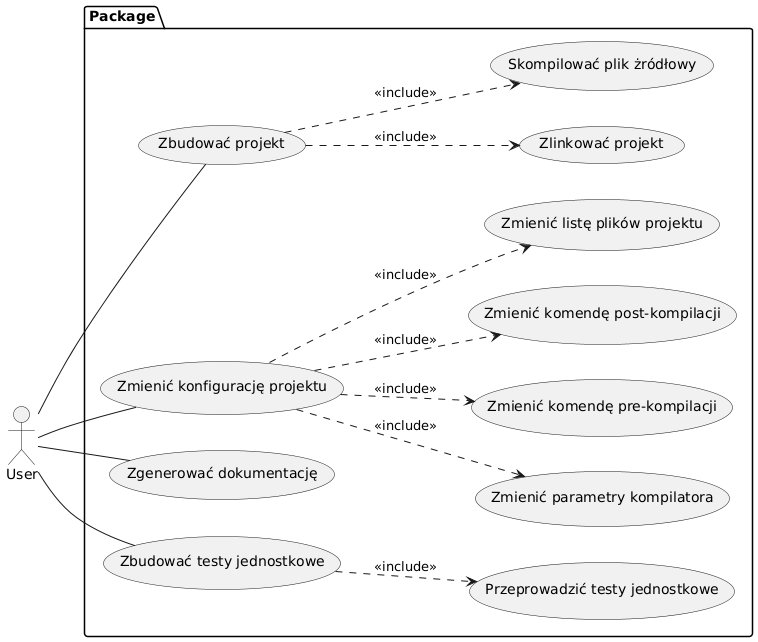
\includegraphics[width=\textwidth]{Images/use-case.png}
    \caption{Przypadki użycia projektu BBS}
\end{figure}

Oprócz wymagań muszą być opisane przypadki użycia programu. Przypadki użycia opisują sekwencje interakcji pomiędzy aktorem (użytkownikiem) a systemem. One są ściśle powiązane z wymaganiami projektowymi i pozwalają wdrożyć tylko i wyłącznie potrzebne funkcje, odrzucając wszystkie inne niewykorzystane funkcje.

Takie podejście nie tylko pozwala usunąć zbędne funkcje, skracając czas realizacji projektu i zmniejszając koszt jego tworzenia, ale też skupia się na użytkownikach.

\subsection{Zbudować projekt (UC1)}
\begin{itemize}
    \item Cel: Umożliwić użytkownikowi pełne zbudowanie projektu, które obejmuje kompilację wszystkich plików źródłowych oraz ich późniejsze połączenie w jeden wynikowy plik wykonywalny lub bibliotekę.
    \item Warunki początkowe: Projekt zawiera poprawnie skonfigurowane pliki źródłowe oraz ustawienia kompilacji.
    \item Warunki końcowe: Projekt został zbudowany.
    \item Scenariusz: 
    \begin{itemize}
    	\item Użytkownik uruchamia program z podaniem pliku konfiguracyjnego.
    	\item System rozpoczyna kompilację plików źródłowych, uruchamiając przypadek użycia „Skompilować plik źródłowy”.
    	\item System przeprowadza proces linkowania, uruchamiając przypadek „Zlinkować projekt”.
    	\item W przypadku braku błędów budowania system zwraca wynikowy plik wykonywalny lub bibliotekę.
    	\item System informuje użytkownika o pomyślnym zakończeniu budowy lub zgłasza ewentualne błędy.
    \end{itemize}
\end{itemize}

\subsection{Skompilować plik źródłowy (UC2)}
\begin{itemize}
    \item Cel: Umożliwić kompilację pojedynczego pliku źródłowego, przekształcając kod źródłowy na kod maszynowy zrozumiały dla komputera.
    \item Warunki początkowe: Plik źródłowy jest dostępny i poprawnie napisany zgodnie z językiem C++.
    \item Warunki końcowe: Plik został skompilowany.
\end{itemize}

\subsubsection{Scenariusz}
\begin{itemize}
    \item System odczytuje wybrany plik źródłowy.
    \item System stosuje ustalone parametry kompilatora do pliku.
    \item System wykonuje proces kompilacji pliku.
    \item W przypadku sukcesu system generuje skompilowany plik obiektowy, informując użytkownika.
    \item W przypadku błędów kompilacji, system zgłasza błędy.
\end{itemize}

\subsection{Zlinkować projekt (UC3)}
\begin{itemize}
    \item Cel: Połączyć wszystkie skompilowane pliki obiektowe w jeden finalny plik wykonywalny lub bibliotekę.
    \item Warunki początkowe: Projekt zawiera co najmniej jeden skompilowany plik obiektowy.
    \item Warunki końcowe: Projekt został zlinkowany.
\end{itemize}

\subsubsection{Scenariusz}
\begin{itemize}
    \item System odczytuje listę plików obiektowych do linkowania.
    \item System wykonuje proces linkowania, tworząc wynikowy plik.
    \item Jeśli linkowanie zakończy się sukcesem, system generuje plik wynikowy i informuje użytkownika.
    \item Jeśli wystąpią błędy, system zgłasza je użytkownikowi.
\end{itemize}

\subsection{Zmienić konfigurację projektu (UC4)}
\begin{itemize}
    \item Cel: Umożliwić użytkownikowi edycję ustawień projektu, co pozwala na dostosowanie jego konfiguracji.
    \item Warunki początkowe: Projekt jest otwarty i posiada dostępne pliki konfiguracyjne.
    \item Warunki końcowe: Konfiguracja projektu została zaktualizowana.
\end{itemize}

\subsubsection{Scenariusz}
\begin{itemize}
    \item Użytkownik otwiera plik konfiguracji projektu.
    \item Użytkownik dokonuje zmian w wybranych ustawieniach.
    \item Użytkownik zapisuje zmiany w konfiguracji projektu.
\end{itemize}

\subsection{Zmienić listę plików projektu (UC5)}
\begin{itemize}
    \item Cel: Pozwala użytkownikowi dodawać lub usuwać pliki źródłowe albo nagłówkowe wchodzące w skład projektu.
    \item Warunki początkowe: Projekt jest otwarty i zawiera aktualną listę plików źródłowych.
    \item Warunki końcowe: Lista plików zmieniona.
\end{itemize}

\subsubsection{Scenariusz}
\begin{itemize}
    \item Użytkownik otwiera plik konfiguracji projektu.
    \item Użytkownik dodaje lub usuwa pliki.
    \item Użytkownik zapisuje zmiany w konfiguracji projektu.
\end{itemize}

\subsection{Zmienić parametry kompilatora (UC6)}
\begin{itemize}
    \item Cel: Umożliwić użytkownikowi dostosowanie parametrów kompilatora, takich jak poziom optymalizacji, ostrzeżenia i inne ustawienia.
    \item Warunki początkowe: Kompilator jest zainstalowany i dostępny w systemie.
    \item Warunki końcowe: pParametry kompilatora zostały zmienione.
\end{itemize}

\subsubsection{Scenariusz}
\begin{itemize}
    \item Użytkownik otwiera plik konfiguracji projektu.
    \item Użytkownik wprowadza zmiany w ustawieniach.
    \item Użytkownik zapisuje zmiany w konfiguracji projektu.
\end{itemize}

\subsection{Zmienić komendę pre-kompilacji (UC7)}
\begin{itemize}
    \item Cel: Umożliwić użytkownikowi ustawienie komend wykonywanych przed kompilacją, np. generacji kodu lub czyszczenia plików tymczasowych.
    \item Warunki początkowe: Projekt jest otwarty, a użytkownik posiada uprawnienia do edycji konfiguracji.
    \item Warunki końcowe: Komenda została zmieniona.
\end{itemize}

\subsubsection{Scenariusz}
\begin{itemize}
    \item Użytkownik otwiera plik konfiguracji projektu.
    \item Użytkownik wprowadza nowe komendy.
    \item Użytkownik zapisuje zmiany w konfiguracji projektu.
\end{itemize}

\subsection{Zmienić komendę post-kompilacji (UC8)}
\begin{itemize}
    \item Cel: Pozwala użytkownikowi skonfigurować komendy, które zostaną wykonane po zakończeniu kompilacji, np. kopiowanie plików wynikowych.
    \item Warunki początkowe: Projekt jest otwarty, a użytkownik posiada uprawnienia do edycji konfiguracji.
    \item Warunki końcowe: Komenda została zmieniona.
\end{itemize}

\subsubsection{Scenariusz}
\begin{itemize}
    \item Użytkownik otwiera plik konfiguracji projektu.
    \item Użytkownik wprowadza nowe komendy.
    \item Użytkownik zapisuje zmiany w konfiguracji projektu.
\end{itemize}

\subsection{Wygenerować dokumentację (UC9)}
\begin{itemize}
    \item Cel: Umożliwić generację dokumentacji projektu na podstawie kodu źródłowego i komentarzy.
    \item Warunki początkowe: Projekt posiada odpowiednie komentarze i strukturę kodu umożliwiającą generowanie dokumentacji.
    \item Warunki końcowe: Dokumentacja została wygenerowana.
\end{itemize}

\subsubsection{Scenariusz}
\begin{itemize}
    \item Użytkownik uruchamia narzędzie generacji dokumentacji.
    \item Doxygen analizuje kod źródłowy i tworzy dokumentację.
    \item Doxygen zapisuje wygenerowaną dokumentację i informuje użytkownika.
\end{itemize}

\subsection{Zbudować testy jednostkowe (UC10)}
\begin{itemize}
    \item Cel: Umożliwić użytkownikowi zbudowanie testów jednostkowych projektu.
    \item Warunki początkowe: Projekt zawiera pliki testowe zgodne z frameworkiem testowym.
    \item Warunki końcowe: Testy jednostkowe zostały zbudowane.
\end{itemize}

\subsubsection{Scenariusz}
\begin{itemize}
    \item Użytkownik wybiera opcję budowy testów jednostkowych.
    \item System buduje testy jednostkowe.
    \item W przypadku braku błędów budowania, system informuje użytkownika o zakończeniu procesu.
\end{itemize}

\subsection{Przeprowadzić testy jednostkowe (UC11)}
\begin{itemize}
    \item Cel: Umożliwić uruchomienie i weryfikację testów jednostkowych w celu sprawdzenia poprawności kodu.
    \item Warunki początkowe: Testy jednostkowe zostały wcześniej zbudowane i są gotowe do uruchomienia.
    \item Warunki końcowe: Wyniki testów jednostkowych zostały zgłoszone użytkownikowi.
\end{itemize}

\subsubsection{Scenariusz}
\begin{itemize}
    \item Użytkownik wybiera opcję uruchomienia testów jednostkowych.
    \item System wykonuje testy i zbiera ich wyniki.
    \item System raportuje wyniki testów, informując użytkownika o przeprowadzonych testach oraz ich rezultatach (sukces lub błąd).
\end{itemize} 
\chapter{Implementacja}
\section{Wprowadzenie}
Celem tego rozdziału jest szczegółowy opis podejścia do realizacji projektu BBS, a mianowicie wyjaśnienie podstawowych pojęć, analiza architektury oraz algorytmów stosowanych do przetwarzania danych.

Chciałbym zacząć od tego, czym właściwie jest BBS. Zgodnie z definicją projekt jest w rzeczywistości procesorem języka \cite{compilers}, a konkretnie tłumaczem według następujących cech, które wynikają bezpośrednio z wymagań opisanych w sekcji 2:
\begin{itemize}
    \item Oprogramowanie analizuje kod wejściowy, napisany w specjalnie opracowanym na potrzeby projektu języku
    \item Oprogramowanie powinno wykrywać i raportować możliwe błędy logiczne lub składniowe w pliku wejściowym
    \item Zamiast tłumaczyć plik wejściowy na inny język programowania, program powinien wykonać polecenia opisane w pliku wejściowym
\end{itemize}

Dodatkowo oprogramowanie to zawiera również preprocesor. Dzieje się tak, aby plik wejściowy mógł zostać podzielony na wiele części, co umożliwi działanie mechanizmu budowania podprojektu.

\section{Struktura interpretera}
Zgodnie ze standardową strukturą kompilatorów i interpreterów, oprogramowanie BBS implementuje część frontend (czyli tę, która przeprowadza analizę) prawie w całości, natomiast backend nie zajmuje się optymalizacją ani generowaniem kodu, ponieważ wykonuje on określone instrukcje na podstawie danych wejściowych (czyli proces syntezy de facto nie zachodzi) \cite{compilers}.

Jeśli patrzyć na dane oprogramowanie ze względu na ogólnie przyjęte fazy kompilacji (które odpowiadają opisanym powyżej częściom standardowego kompilatora lub interpretera), to BBS realizuje prawie wszystkie fazy frontendu, z wyjątkiem generowania kodu pośredniego. Wynika to z niepraktyczności generowania kodu pośredniego bez znaczących opcji jego dalszego wykorzystania. Więc BBS zamiast tej fazy ma swoją, specjalną fazę - fazę wypełniania wewnętrznej struktury opisującej projekt, który ma zostać zbudowany z BBS. Sama konstrukcja, a także procesy zachodzące w tej fazie zostaną szczegółowo opisane w dalszej części.

Podejście do implementacji backendu zasadniczo różni się od standardowego: nie jest wymagane dalsze tłumaczenie kodu na inny język, nie są realizowane fazy generowania kodu w innym języku. Zamiast tego backend na podstawie informacji o projekcie dostarczonych użytkownikowi wybiera określone polecenia do kontrolowania i budowania projektów.

Schemat fazowy BBS wygląda następująco:

\begin{figure}[h]
    \caption{Schemat fazowy projektu BBS}
    \centering
    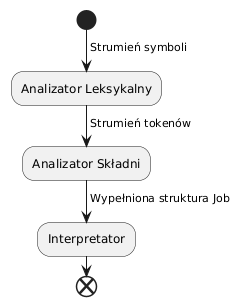
\includegraphics[width=0.4\textwidth]{Images/phases.png}
\end{figure}

Następnie opis procesu implementacji programu zostanie podzielony na części, które również dzielą się na fazy. Ma to na celu proste opisanie procesów zachodzących w środku programu, a także zademonstrowanie danych wejściowych/wyjściowych.

\section{Analiza}
Jak opisano powyżej, dane wejściowe są analizowane w części frontendowej programu. Analizator dzieli dane wejściowe na części i narzuca im strukturę gramatyczną, która później posłuży do zbudowania projektu. Jeżeli parser stwierdzi, że dane wejściowe są niepoprawne składniowo lub semantycznie, informuje o tym użytkownika w najbardziej zrozumiały sposób. Dodatkowo analizator zbiera informacje w postaci tablicy symboli, co zostanie opisane w dalszej części.

\subsection{Analiza leksykalna}
Analiza leksykalna jest pierwszym etapem analizy danych wejściowych. Analizator leksykalny odczytuje strumień symboli i grupuje je w sensowną sekwencję zwaną leksemami, dla których analizator leksykalny generuje tzw. token składający się z typu pary -- odwołanie do tabeli symboli \cite{compilers}.

W projekcie BBS analizator leksykalny jest podzielony na dwie odrębne klasy, \texttt{Lexer} i \texttt{Scanner}, dla których zaimplementowana jest także klasa pomocnicza \texttt{Context}. Także klasy te korzystają z dodatkowych elementów, które zostaną opisane później (ale będą tu omawiane tylko te, które naprawdę zasługują na uwagę, np. nie będzie tu opisu klas wyjątków).

\subsubsection{Klasa Scanner}
Klasa \texttt{Scanner} jest osobną klasą, której delegowana jest rola odczytu plików. To właśnie w tej klasie hermetyzowane są wszelkie operacje sprawdzania istnienia, otwierania i odczytywania plików znak po znaku, a także omijania pustych linii czy komentarzy. Jego implementacja jest dość prosta, gdyż \texttt{Scanner} umożliwia odczytanie bieżącego znaku (funkcja \texttt{Get()}) i przejście do następnego (funkcja \texttt{Move()}). Z kolei operacja \texttt{Get()} opiera się na \texttt{std::optional} \cite{cpp_optional}, innowacji w C++17, która pozwala przechowywać wartość lub nic w bezpieczny i przejrzysty sposób. Klasa na wejściu otrzymuje nazwę pliku do odczytania, a na wyjściu zwraca przeczytany znak (odfiltrowując niepotrzebne), jeśli takie istnieją.

Na szczególną uwagę zasługuje metoda o nazwie \texttt{Skip()} (wywoływana wewnątrz metody \texttt{Move()}), która wykonuje operację pomijania komentarzy i pustych znaków w przypadku konieczności przeczytania kolejnej linii (czyli oznacza, że został znaleziony znak nowej linii). Ta metoda wygląda następująco:

\begin{lstlisting}[label=list:scanner,caption=Metoda Scanner::Skip(),basicstyle=\footnotesize\ttfamily]
void Scanner::Skip()
{
    // Read the next line if scanner finds a new line symbol, a comment or an empty line
    auto character = context_.GetCharacter();
    while(!character || character.value() == constants::kComment)
    {
        std::string line;
        std::getline(file_, line);
        if(file_.fail())
        {
            file_.close();
            return;
        }
    
        context_.Update(std::move(line));
        character = context_.GetCharacter();
    }
    
    // Check if the line still has anything to read
    if(!character || character.value() == '\0')
    {
        file_.close();
    }
}
\end{lstlisting}

Analizując ten kod, możemy stwierdzić, że \texttt{Scanner} najpierw odczytuje bieżący znak, który następnie przechodzi sprawdzenie istnienia (\texttt{std::optional} jest pusty, jeśli znak nie był czytany przez zamknięty plik, np.) lub równość określonego w gramatyce języka symbolu komentarza. Następnie, w przypadku pozytywnego wyniku kontroli (pusty znak lub komentarz), \texttt{Scanner} próbuje odczytać następną linię. Jeśli instrukcja się powiedzie, \texttt{Scanner} aktualizuje kontekst nową linią i zapamiętuje nowy znak jako bieżący, po czym powtarzane jest sprawdzenie istnienia znaku lub komentarza (ponieważ nowa linia może zawierać także komentarz). Przy wyjściu z pętli \texttt{Scanner} sprawdza, czy ostatnia linia została odczytana i jeśli odpowiedź jest pozytywna, plik jest zamykany.

\subsubsection{Klasa Context}
Między innymi moduł \texttt{lexer} zawiera ważną klasę pomocniczą \texttt{Context}, której wpływ na moduł jest dość znaczący. Klasa ta pojawiła się w procesie rozbudowy i rozwoju projektu BBS poprzez wyodrębnienie metod i pól z klasy \texttt{Scanner} w celu nie tylko spełnienia zasad SOLID \cite{solid}, ale także ułatwienia dostępu do informacji o bieżącej lokalizacji w pliku. Funkcjonalność ta służy w szczególności szczegółowemu informowaniu użytkownika o błędach składniowych lub semantycznych.

Klasa \texttt{Context} zawiera bieżącą linię przetwarzaną przez program, jej indeks w pliku oraz pozycję bieżącego znaku w linii. Wszystkie pola są chronione i dostępne pośrednio poprzez predefiniowany interfejs.

\subsubsection{Klasa Lexer}
Klasa \texttt{Lexer}, jak sama nazwa wskazuje, jest implementacją analizatora leksykalnego. Ta klasa jest najbardziej złożona ze wszystkich w module, a jej struktura jest modułowa, co ułatwia zmianę jej elementów w miarę zmiany wymagań lub gramatyki języka.

Główna klasa \texttt{Lexer} ma tylko metody manipulacji tokenami (\texttt{Get()} do odczytania bieżącego tokena i \texttt{Next()} do żądania odczytania następnego tokena), ponieważ praca z plikami została delegowany do klasy \texttt{Scanner}.

Proces kategoryzacji tokenów został delegowany do szeregu klas zwanych procedurami obsługi. Klasy te stanowią implementację wzorca projektowego „Łańcuch odpowiedzialności” \cite{cor}, który polega na przetwarzaniu określonych żądań przez dany obiekt i ich późniejszym przekazywaniu do kolejnych obiektów, w przypadku gdyby żądanie nie powiodło się. Ten wzorzec został użyty, aby wycofać użycie \texttt{switch-case}, aby umożliwić znacznie łatwiejsze (i jednolite) podłączanie nowych klas obsługi przy minimalnych zmianach w istniejącym kodzie (zgodnie z zasadami SOLID \cite{solid}). Klasy te posiadają następujący interfejs:

\begin{lstlisting}[label=list:handler,caption=Klasa Handler,basicstyle=\footnotesize\ttfamily]
/**
 * @brief A default Lexer input handler, an implementation of the CoR pattern
 * 
 */
class Handler
{
    using Token = parser::tokens::Token;
    
public:
    /**
     * @brief Process the input and return the token if possible
     * 
     * @param scanner - the source of characters to process
     * @return std::unique_ptr<Token> - a pointer to the token or nullptr 
     */
    virtual std::unique_ptr<Token> Process(Scanner& scanner) const;
    
    /**
     * @brief Set the next handler to be called to process the input
     * 
     * @param next - a pointer to the next handler to be called
     */
    void SetNext(std::unique_ptr<Handler> next);
    
protected:
    /**
     * @brief A pointer to the handler, next on the line to process the input
     * 
     */
    std::unique_ptr<Handler> next_;
};
\end{lstlisting}

Oznacza to, że każdy obiekt przetwarzający po utworzeniu otrzymuje łącze do następcy, do którego zostanie przekazane żądanie w przypadku niepowodzenia podczas jego realizacji. Jeśli żaden z programów obsługi nie był w stanie przetworzyć żądania, ostatni w łańcuchu tworzy wyjątek. Implementacja ta pozwoliła maksymalnie uprościć klasę \texttt{Lexer}, kod metody \texttt{Next()}, która wymusza na parserze odczytanie kolejnego tokena z pliku, dzięki wzorcowi "łańcuch odpowiedzialności" \cite{cor} został uproszczony do następującej postaci bez poświęcania stabilności i bezpieczeństwa programu:

\begin{lstlisting}[label=list:scanner,caption=Metoda Lexer::Next(),basicstyle=\footnotesize\ttfamily]
std::shared_ptr<Lexer::Token> Lexer::Next()
{
    token_ = std::move(handler_->Process(scanner_));
    return token_;
}
\end{lstlisting}

Klasa \texttt{Lexer} na wejściu otrzymuje nazwę pliku (która jest przekazywana do obiektu klasy Scanner i nie jest zapisywana bezpośrednio), na wyjściu \texttt{Lexer} zwraca aktualny token, a także umożliwia odczytanie nowy. W przypadku znalezienia nieznanych symboli, których nie przewidywała gramatyka języka, analizator tworzy odpowiedni wyjątek ze szczegółowym opisem położenia symbolu i przyczyną błędu.

Lista tokenów, które program może przetworzyć, odpowiada podanemu językowi i została opisana w sekcji ''Gramatyk języka''.
\chapter{Wnioski}
Praca nad projektem BBS umożliwiła stworzenie narzędzia, które usprawnia proces budowania projektów w języku C++. Automatyzacja kompilacji, linkowania oraz zarządzania zależnościami pozwala znacząco uprościć pracę programistów, szczególnie w przypadku dużych i złożonych projektów.

Analiza dostępnych narzędzi, takich jak \textbf{Make}, \textbf{CMake}, \textbf{NMake} czy \textbf{Meson}, wykazała, że każde z nich ma swoje mocne strony, jednak mogą być one trudne w użyciu lub nadmiarowe w stosunku do wymagań mniejszych projektów. BBS celuje w dostarczenie intuicyjnego i wydajnego rozwiązania, które eliminuje te problemy.

Wnioski z pracy nad tym projektem obejmują:
\begin{itemize}
    \item Znaczenie automatyzacji: Automatyzacja procesu budowania, szczególnie w przypadku dużych projektów, pozwala uniknąć błędów, oszczędza czas i zwiększa produktywność zespołów programistycznych.
    \item Znaczenie czytelności kodu i dokumentacji: Korzystanie z takich narzędzi jak Doxygen i clang-format wspiera utrzymanie standardów kodu, co ułatwia pracę nad projektem zarówno obecnym, jak i przyszłym członkom zespołu.
    \item Rozwijanie standardów w C++: Nowoczesne cechy języka, takie jak std::filesystem czy std::optional, znacząco upraszczają implementację i poprawiają czytelność kodu.
\end{itemize}

Projekt BBS pokazuje, że możliwe jest stworzenie narzędzia do budowania projektów w C++, które jest lekkie, wydajne i łatwe w użyciu. Dalsze kierunki rozwoju obejmują dodanie wsparcia dla bardziej zaawansowanych funkcji, takich jak dużo lepsze raportowanie błędów z pięknym formatowaniem, lepsze zarządzanie wątkami i jednoczesne budowanie kilku projektów, rozszerzenie listy wspieranych języków i kompilatorów oraz integracja z istniejącymi IDE (np. Visual Studio).

Realizacja tego projektu pozwoliła na zdobycie praktycznych umiejętności z zakresu nowoczesnego C++, inżynierii oprogramowania (w szczególności kompilatorów i interpreterów) oraz pracy z narzędziami wspierającymi rozwój dużych projektów. Wyniki pracy mogą być z powodzeniem wykorzystane jako fundament dla przyszłych projektów czy w celu zastąpienia innych rozwiązań nowoczesnym, wydajnym i łatwym w obsłudze oprogramowaniem.
% LITERATURA (zostanie wygenerowana automatycznie)
%UWAGA: bibliotekę referencji należy przygotować samemu. Dobrym do tego narzędziem jest JabRef.
%       JabRef oferuje jednak większą liczbę typów rekordów niż obsługuje BibTeX.
%       Proszę nie deklarować rekordów o typach nieobsługiwanych przez BibTeX.
%       Formatowania wykazu literatury i cytowań odbywać się ma zgodnie z zadeklarowanym stylem.
%       Zalecane są style produkujące numeryczne cytowania (w postaci [1], [2,3]).
%       Takim stylem jest np. plabbrv
\bibliographystyle{plabbrv}
%       Aby zapanować nad odstępami w wykazie literatury można posłużyć się poniższą komendą
\setlength{\bibitemsep}{2pt} % - zacieśnia wykaz
%       Pozycja Literatura pojawia się w spisie treści nieco inaczej niż spisy rysunków, tabel itp.
%       Aby zachować właściwe odstępy należy użyć poniższej komendy
\addtocontents{toc}{\addvspace{2pt}} % ustawiamy odstęp w spisie treści przed pozycją Literatura 
%       Nazwę pliku przygotowanej biblioteki wpisuje się bez rozszerzenia .bib
%       (linia poniżej załaduje rekordy z pliku "dokumentacja.bib")
\bibliography{dokumentacja}
\appendix
\chapter{Instrukcja wdrożeniowa}
Jeśli praca skończyła się wykonaniem jakiegoś oprogramowania, to w dodatku powinna pojawić się instrukcja wdrożeniowa (o tym jak skompilować/zainstalować to oprogramowanie).
Przydałoby się również krótkie ,,\emph{how to}'' (jak uruchomić system i coś w nim zrobić -- zademonstrowane na jakimś najprostszym przypadku użycia). Można z tego zrobić osobny dodatek.
\chapter{Instrukcja Obsługi}

Poniżej znajduje się instrukcja uruchomienia aplikacji BBS oraz opis formatu pliku konfiguracyjnego wykorzystywanego do definiowania procesu budowy.

\section{Proces uruchomienia}

Aby uruchomić aplikację BBS, należy wykonać następujące kroki:

\begin{enumerate}
	\item Przygotuj plik konfiguracyjny w formacie tekstowym, opisujący szczegóły projektu, takie jak nazwa projektu, pliki źródłowe, biblioteki zależne, flagi kompilatora itp.
	\item W terminalu przejdź do katalogu, w którym będzie się znajdował zbudowany projekt.
	\item Uruchom aplikację, podając jako argument ścieżkę do pliku konfiguracyjnego. Przykładowa komenda:
	\begin{lstlisting}
	./bbs ..
	\end{lstlisting}
	\item Aplikacja rozpocznie proces budowy projektu zgodnie z definicjami zawartymi w pliku konfiguracyjnym. W terminalu będą wyświetlane informacje o postępie.
\end{enumerate}
\section{Format pliku konfiguracyjnego}

Plik konfiguracyjny w BBS jest oparty na prostym formacie tekstowym, w którym definiowane są wszystkie aspekty projektu. Poniżej znajduje się szczegółowy opis słów kluczowych używanych w tym pliku:

\paragraph{\texttt{!let}} Pozwala na definiowanie zmiennych, które mogą być wykorzystywane w innych sekcjach pliku. Zmienna musi mieć unikalną nazwę oraz wartość w formie ciągu znaków.
\begin{lstlisting}[language=sh,alsoletter={!},keywords={!let,!prj,!files,!deps,!cflags,!pre,!post,!inc},keywordstyle=\bfseries]
!let project_name = "MyApp"
\end{lstlisting}

\paragraph{\texttt{!prj}} Definiuje nazwę projektu. Może zawierać bezpośrednią wartość lub odwołanie do zmiennej.
\begin{lstlisting}[language=sh,alsoletter={!},keywords={!let,!prj,!files,!deps,!cflags,!pre,!post,!inc}]
!prj "MyApp"
!prj $project_name
\end{lstlisting}

\paragraph{\texttt{!files}} Określa listę plików źródłowych do skompilowania. Pliki są umieszczone w nawiasach kwadratowych, oddzielone przecinkami i ujęte w cudzysłowy.
\begin{lstlisting}[language=sh,alsoletter={!},keywords={!let,!prj,!files,!deps,!cflags,!pre,!post,!inc}]
!files [ "main.cpp", "utils.cpp", "app.cpp" ]
\end{lstlisting}

\paragraph{\texttt{!deps}} Definiuje projekty zależne, które powinny zostać zbudowane przed głównym projektem. Musi być podana względna ścieżka do tych projektów.
\begin{lstlisting}[language=sh,alsoletter={!},keywords={!let,!prj,!files,!deps,!cflags,!pre,!post,!inc}]
!deps [ "dependency" ]
\end{lstlisting}

\paragraph{\texttt{!cflags}} Określa flagi kompilatora, takie jak opcje optymalizacji, ostrzeżenia czy inne parametry.
\begin{lstlisting}[language=sh,alsoletter={!},keywords={!let,!prj,!files,!deps,!cflags,!pre,!post,!inc}]
!cflags "-O2 -Wall -lsomelib"
\end{lstlisting}

\paragraph{\texttt{!pre}} Definiuje polecenia do wykonania przed rozpoczęciem procesu kompilacji, np. wyświetlenie komunikatu w terminalu.
\begin{lstlisting}[language=sh,alsoletter={!},keywords={!let,!prj,!files,!deps,!cflags,!pre,!post,!inc}]
!pre "echo 'Rozpoczynam budowanie projektu...'"
\end{lstlisting}

\paragraph{\texttt{!post}} Definiuje polecenia wykonywane po zakończeniu procesu kompilacji, np. informowanie o sukcesie lub kopiowanie plików.
\begin{lstlisting}[language=sh,alsoletter={!},keywords={!let,!prj,!files,!deps,!cflags,!pre,!post,!inc}]
!post "echo 'Budowanie zakończone!'"
\end{lstlisting}

\paragraph{\texttt{!inc}} Określa ścieżki do katalogów z plikami nagłówkowymi wymaganymi w procesie kompilacji.
\begin{lstlisting}[language=sh,alsoletter={!},keywords={!let,!prj,!files,!deps,!cflags,!pre,!post,!inc}]
!inc [ "include/", "external/includes/" ]
\end{lstlisting}

Każde z tych słów kluczowych jest integralną częścią procesu budowy projektu w BBS, umożliwiając elastyczną kontrolę nad kompilacją i konfiguracją projektu. Przygotowując plik konfiguracyjny zgodnie z opisanymi wytycznymi, można w pełni wykorzystać możliwości tego narzędzia.

\section{Działanie aplikacji}
Po uruchomieniu aplikacja odczytuje plik konfiguracyjny i realizuje zdefiniowane w nim kroki. Proces ten obejmuje:

\begin{itemize}
    \item Sprawdzenie, czy wszystkie pliki źródłowe i katalogi istnieją.
    \item Przygotowanie flag i parametrów kompilatora.
    \item Kompilację plików źródłowych i ich linkowanie do postaci programu wykonywalnego.
    \item Wykonanie poleceń określonych w sekcjach pre i post, jeśli zostały podane.
\end{itemize}

Jeśli podczas budowania projektu wystąpią błędy, takie jak brak plików źródłowych lub nieprawidłowa składnia w pliku konfiguracyjnym, aplikacja zgłasza je w formie komunikatów błędów w terminalu.

% Jeśli w pracy pojawiać się ma indeks, należy odkomentować poniższe linie
%%\chapterstyle{noNumbered}
%%\phantomsection % sets an anchor
%%\addcontentsline{toc}{chapter}{Indeks rzeczowy}
%%\printindex

\end{document}
